\indent\textbf{Цель работы:} изучить спектры сигналов различной формы и влияние параметров сигнала на вид соответствующих спектров; проверить справедливость соотношений неопределённостей; познакомиться с работой спектральных фильтров на примере RC-цепочки.\\\indent
\textbf{Оборудование:} генератор сигналов произвольной формы, цифровой осциллограф с функцией быстрого преобразования Фурье или цифровой USB-осциллограф, подключённый к персональному компьютеру.\\
\subsection*{Исследование спектра периодической последовательности прямоугольных импульсов и проверка соотношений неопределенности}

\begin{figure}[h!]
    \centering
    \begin{subfigure}{.6\linewidth}
        \centering
        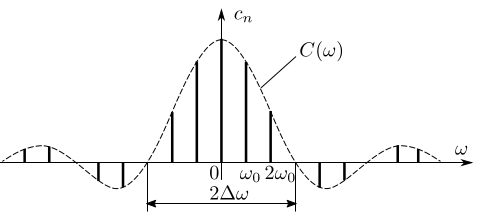
\includegraphics[width=8cm]{images/spectr.png}
    \end{subfigure}
    \hfill
    \begin{subfigure}{.39\linewidth}
        \centering
        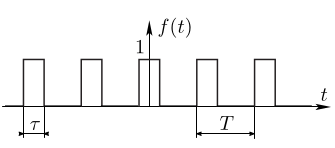
\includegraphics[width=6cm]{images/periodic_signals.png}
    \end{subfigure}
    \caption{Периодическая последовательность импульсов и её спектр}
\end{figure}
Найдем спектр периодической последовательности прямоугольных импульсов длительности $\tau$ и периодом следования импульсов $T > \tau$:
\begin{equation}
    c_n = \frac{1}{T}\int_{-\tau / 2}^{\tau / 2} e^{-in\omega_0t}dt = \frac{\tau}{T}\cdot\frac{\sin({\pi n \tau / T)}}{n\omega_0 \tau / 2} = \frac{\sin(\pi n\tau /T) }{\pi n}
\end{equation}
\indent Тогда представленные ниже фотографии лекго объяснить. При увеличении частоты повторения синус растет, а с ним и амплитуда гармоник. При этом кол-во гармоник в полуширине уменьшается т.к частота повторения растет. Если же увеличивать длительность импульса, то амплитуда гармоник растет, а ширина $\Delta \omega$ уменьшается.
\newpage
\begin{figure}[h!]
    \centering
    \begin{subfigure}[b]{0.3\linewidth}
        \centering
        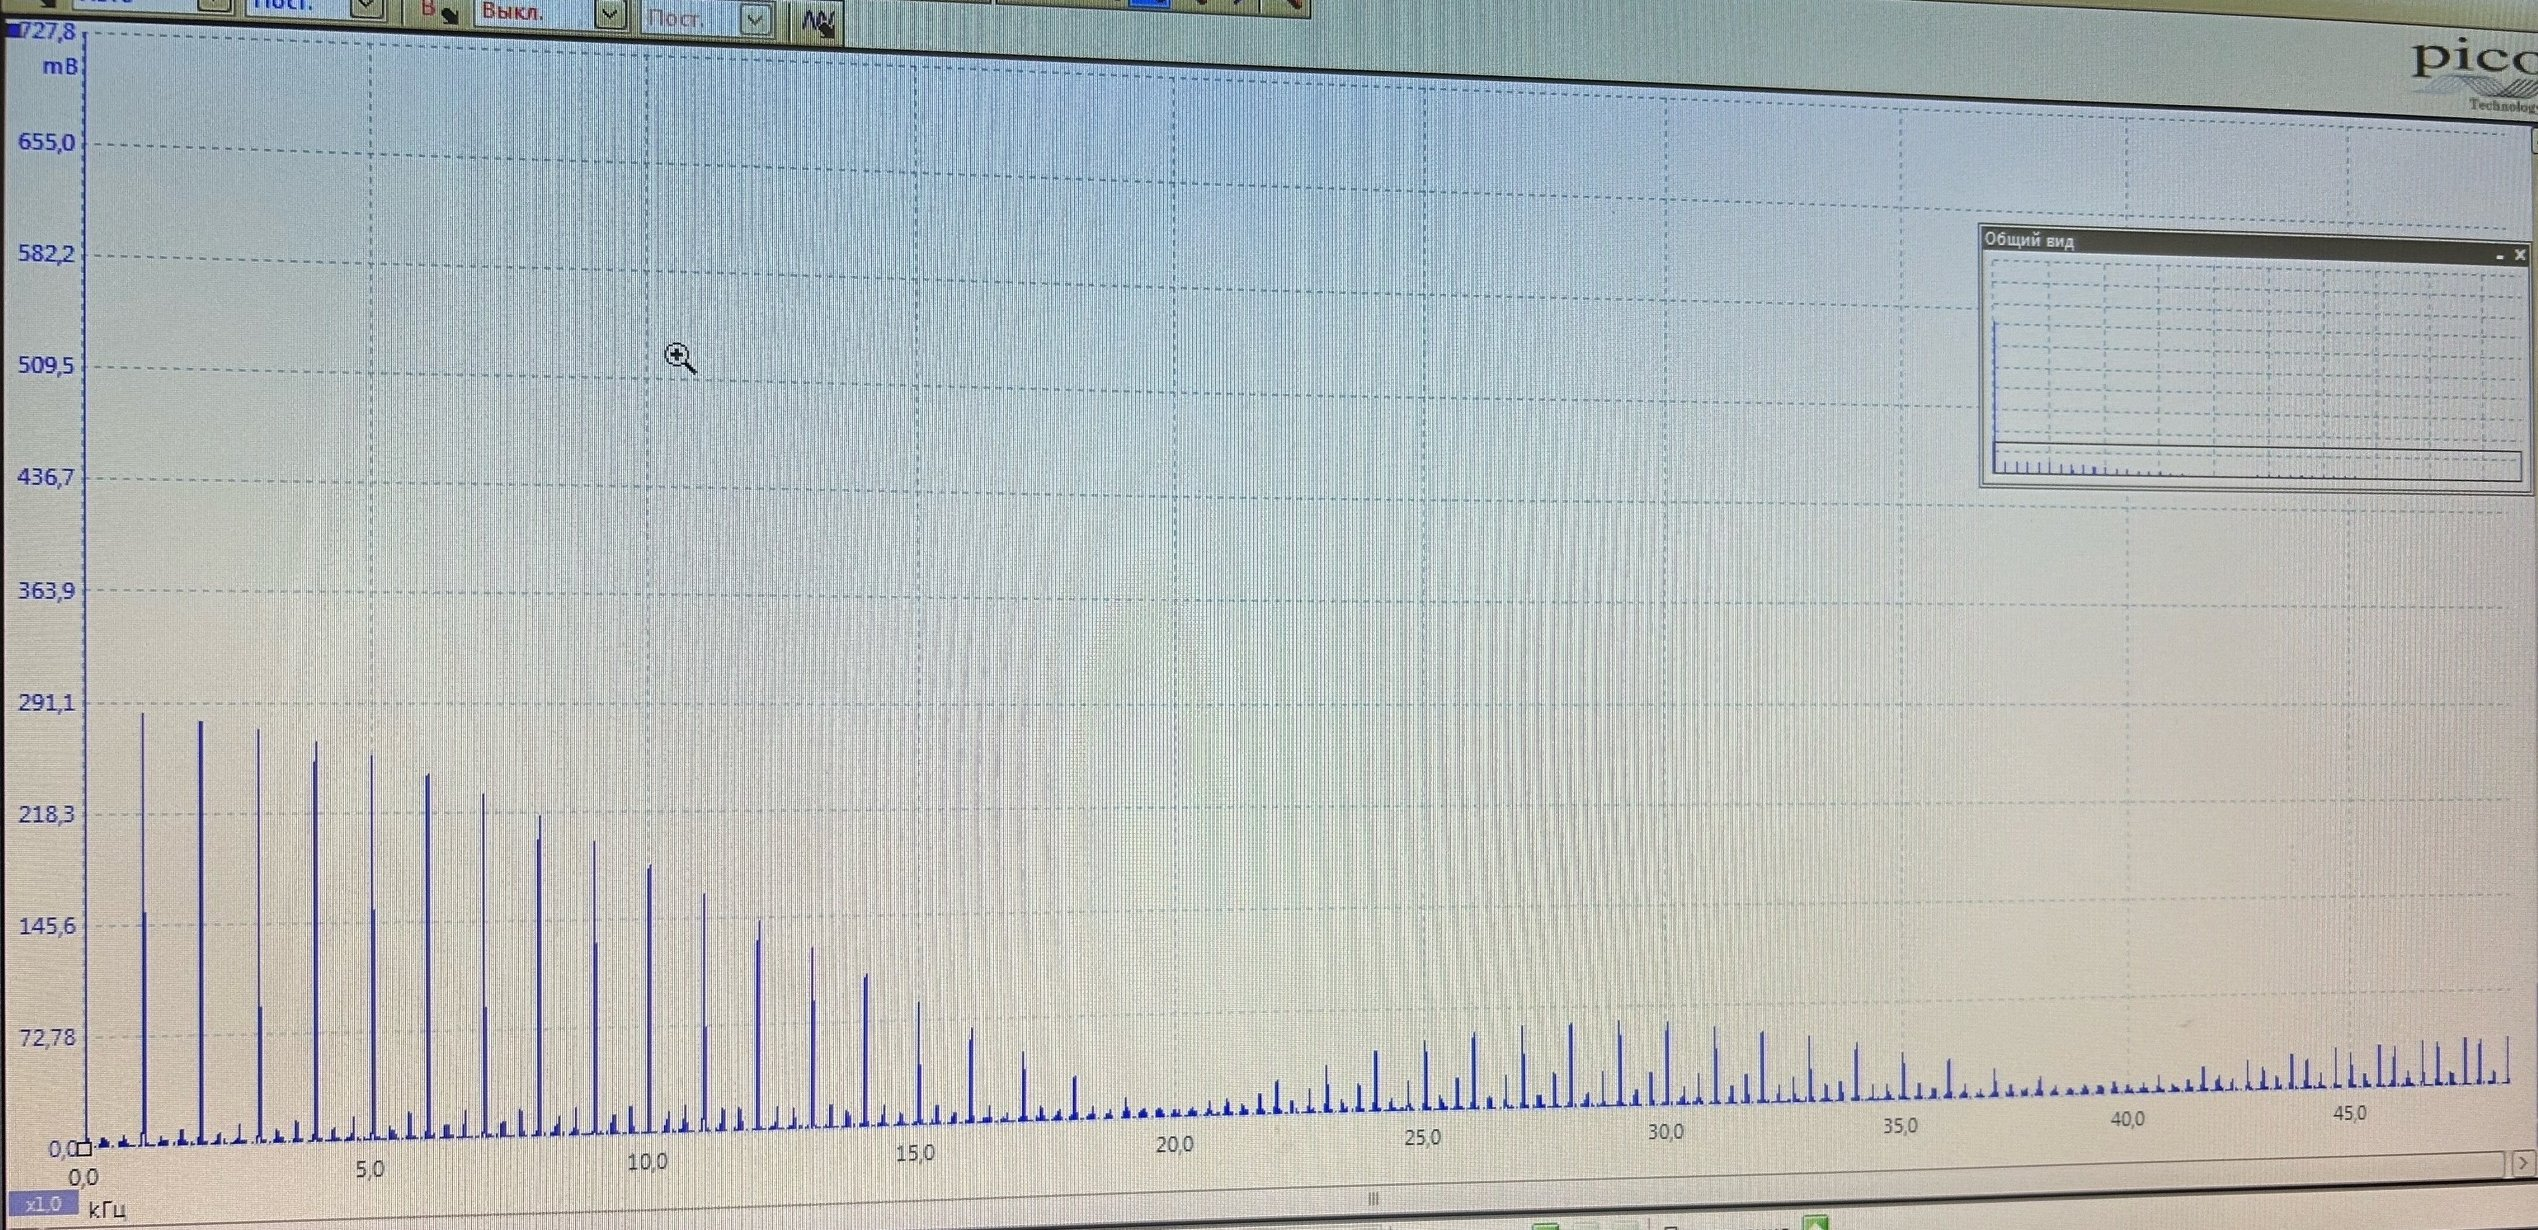
\includegraphics[width=6cm]{./images/nu_1_t_50.jpg}
        \caption{$\nu_{\text{повт}} = 1$кГц; $\tau = 50$ мкс}
    \end{subfigure}
    \hfill
    \begin{subfigure}[b]{0.3\linewidth}
        \centering
        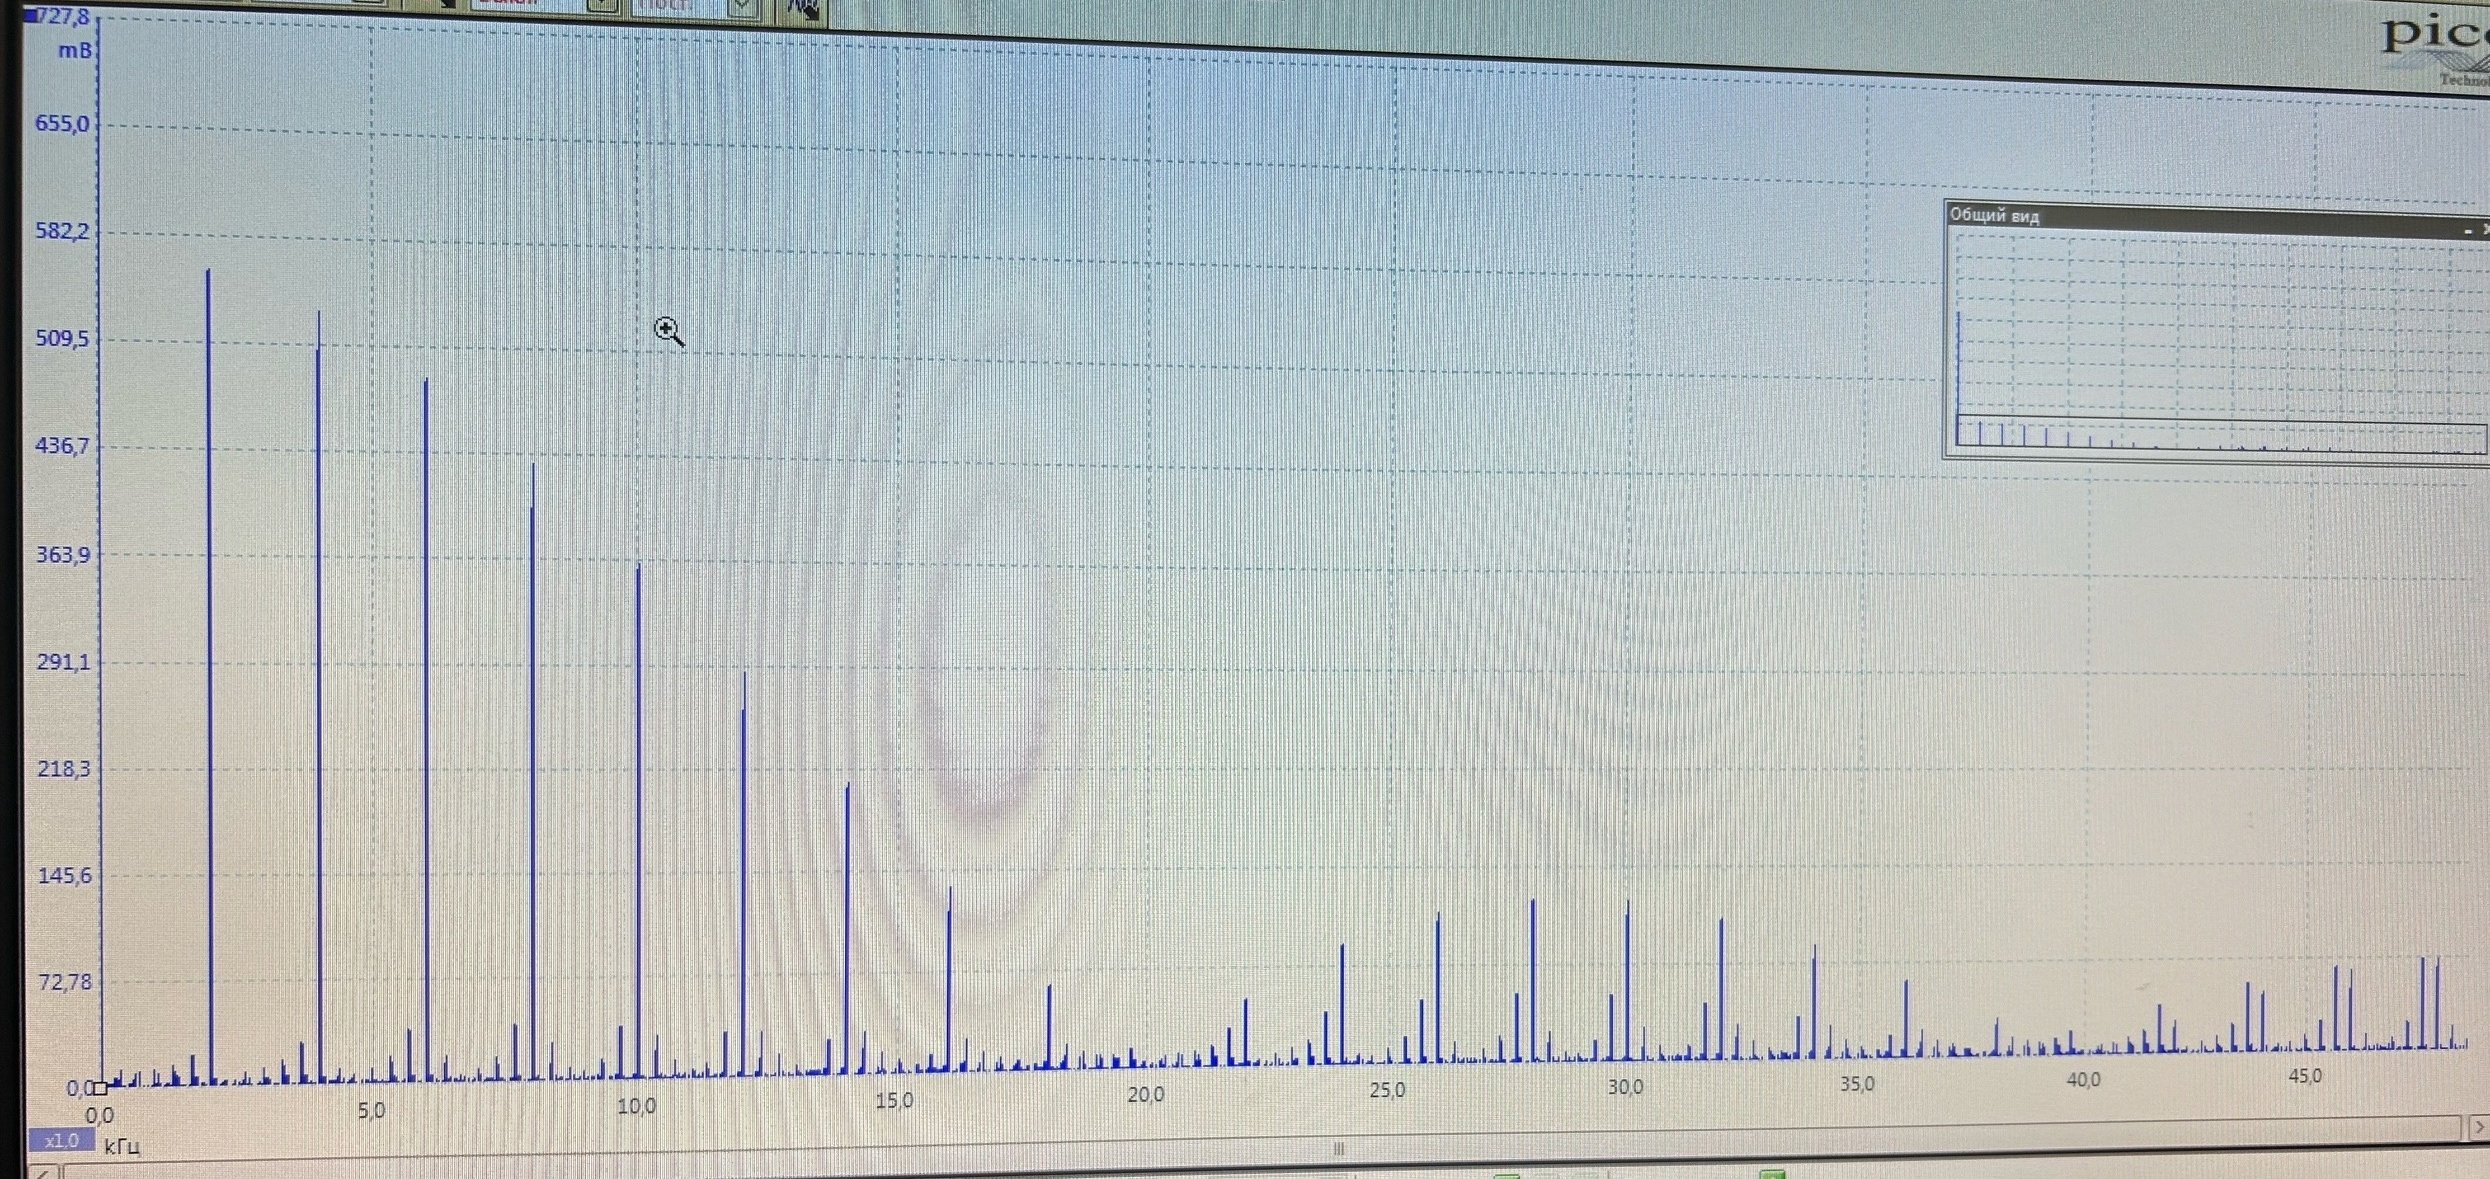
\includegraphics[width=6cm]{./images/nu_2_t_50.jpg}
        \caption{$\nu_{\text{повт}} = 2$кГц; $\tau = 50$ мкс}
    \end{subfigure}
    \hfill
    \begin{subfigure}{0.3\linewidth}
        \centering
        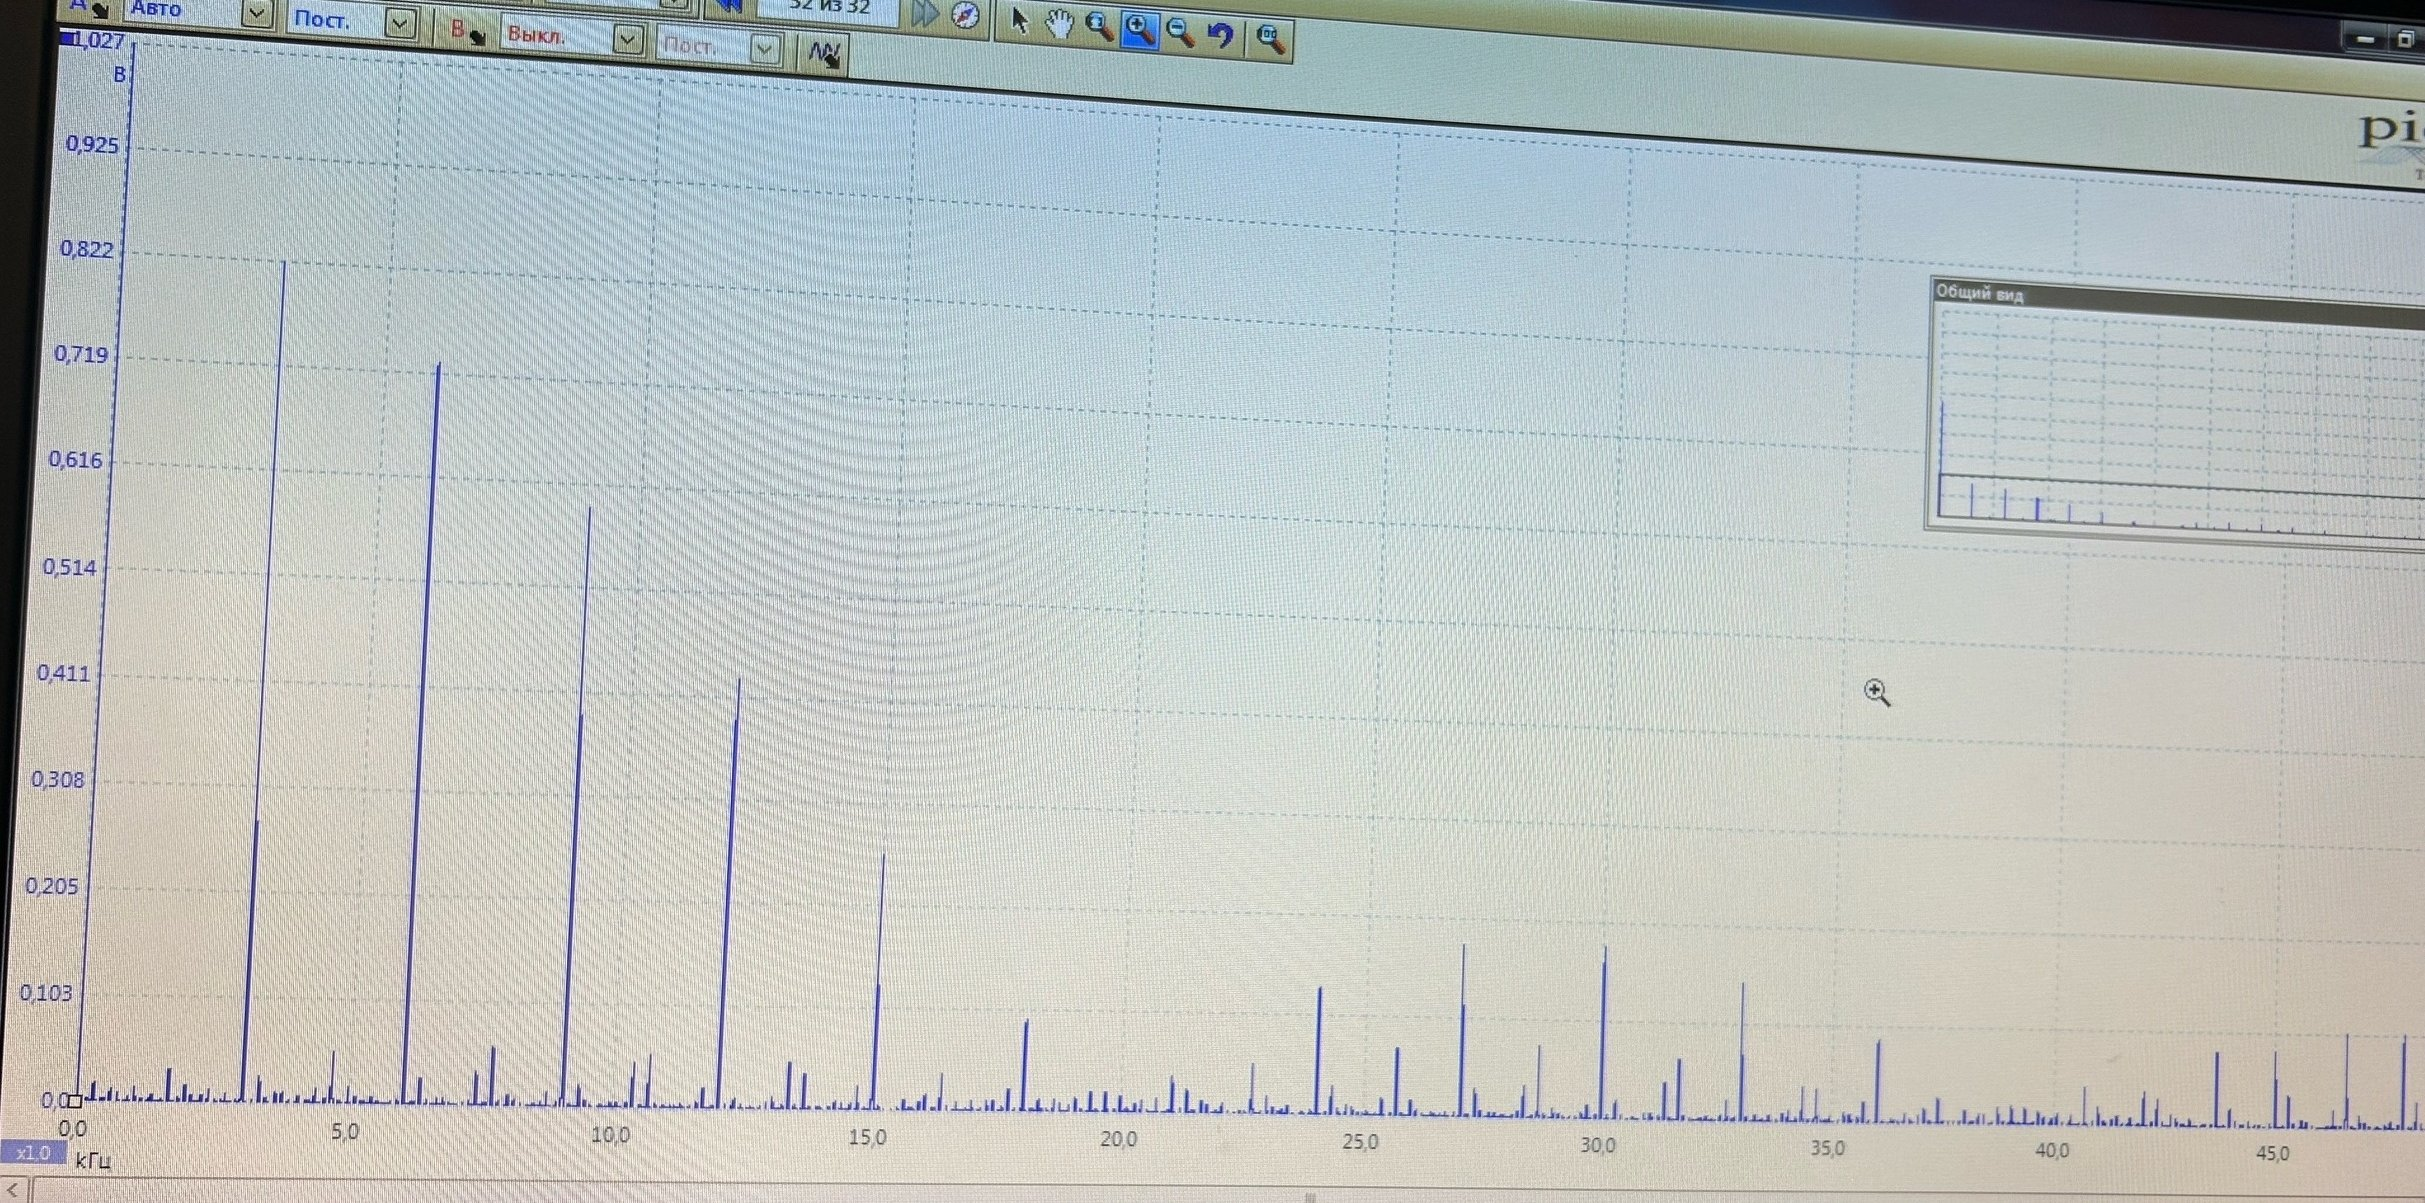
\includegraphics[width=6cm]{./images/nu_3_t_50.jpg}
        \caption{$\nu_{\text{повт}} = 3$кГц; $\tau = 50$ мкс}
    \end{subfigure}
    \vfill
    \begin{subfigure}{0.35\linewidth}
        \centering
        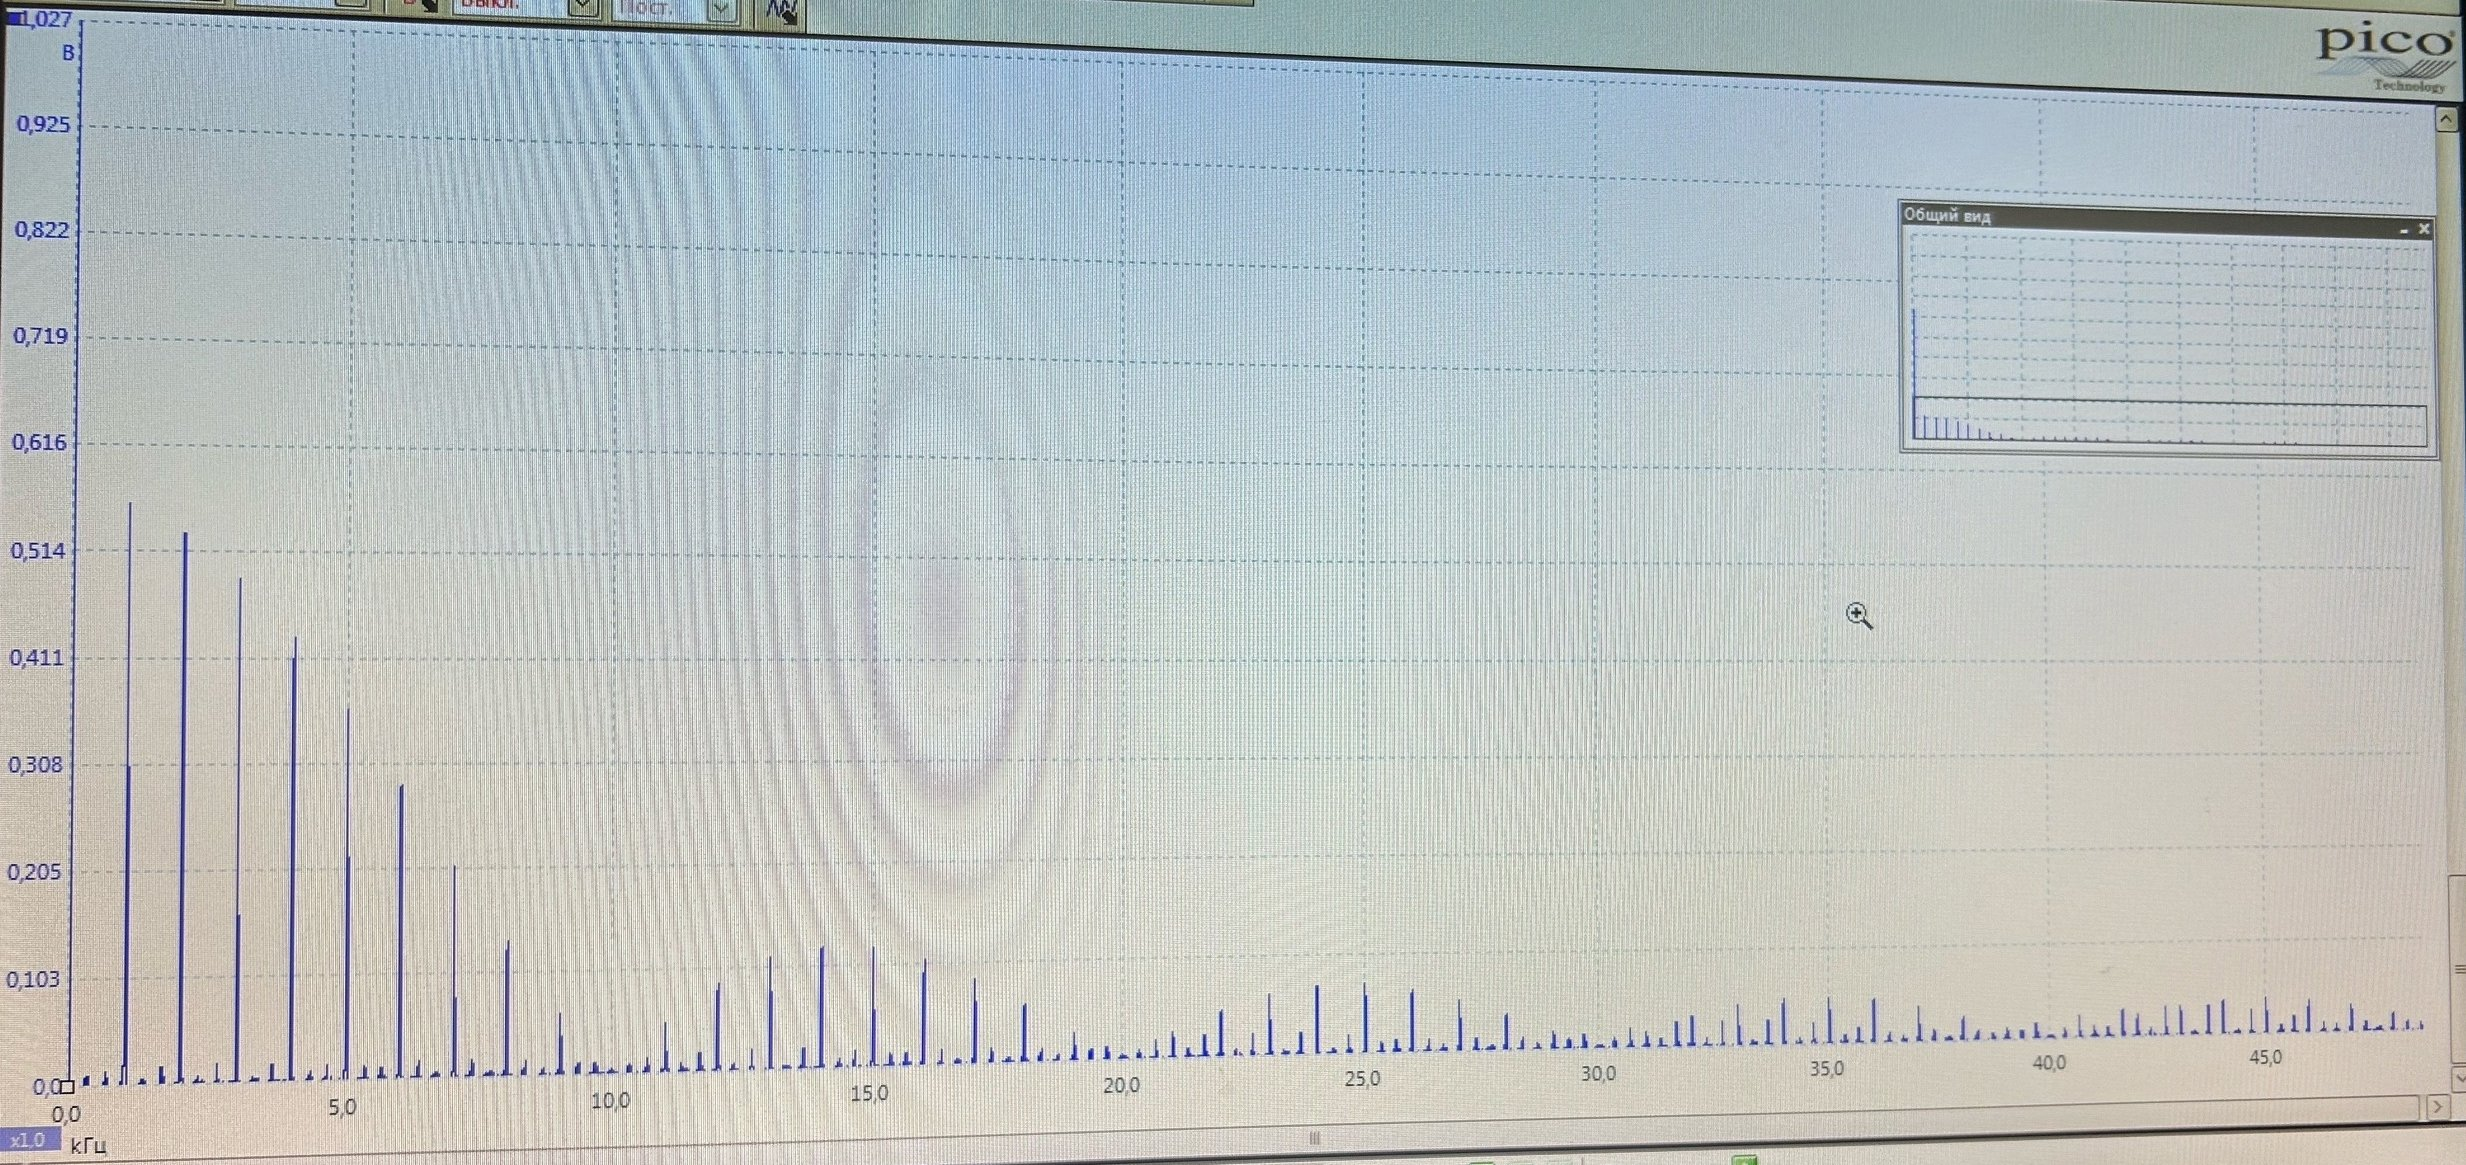
\includegraphics[width=6cm]{./images/nu_1_t_100.jpg}
    \caption{$\nu_{\text{повт}} = 1$кГц; $\tau = 100$ мкс}
    \end{subfigure}
    \begin{subfigure}{0.35\linewidth}
        \centering
        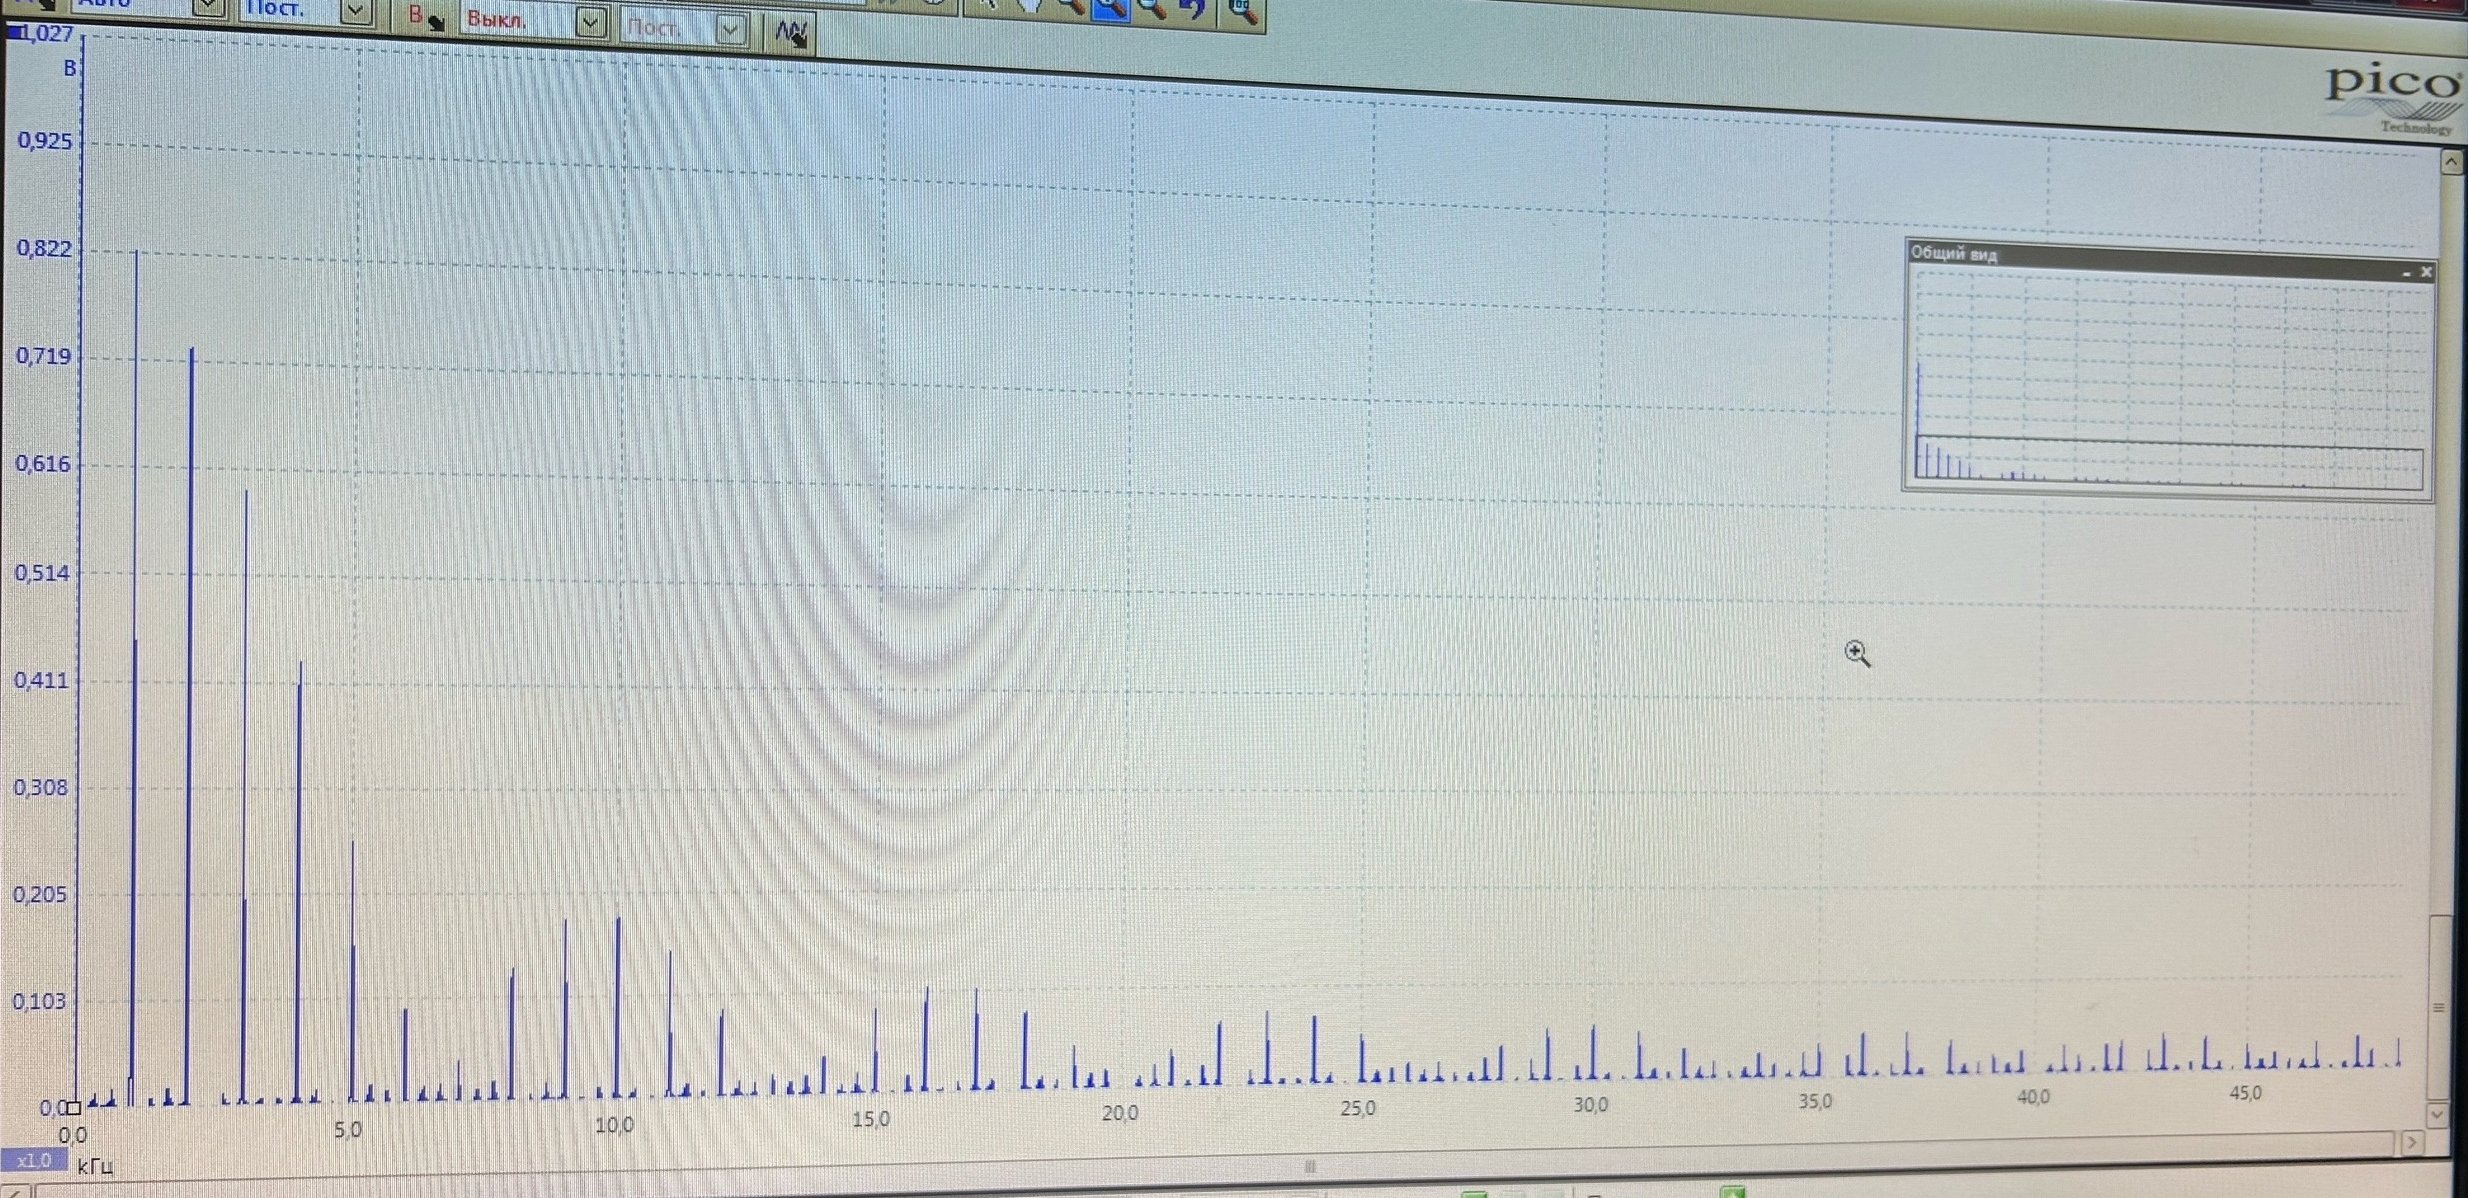
\includegraphics[width=6cm]{./images/nu_1_t_150.jpg}
    \caption{$\nu_{\text{повт}} = 1$кГц; $\tau = 150$ мкс}
    \end{subfigure}
    \caption{Изменения спектров при разных параметрах сигнала}
\end{figure}

\begin{table}[h!]
    \centering
    \begin{tabular}{|c|c|c|c|c|c|c|}
        \hline
        $n$ & 1 & 3 & 8 & 9 & 12 & 15\\\hline
        $\nu_n$, кГц & 1 & 3 & 9 & 10 & 12 & 15\\\hline 
        $|a_n|$, усл.ед & 282.6 & 274 & 196.9 & 179.8 & 145.6 & 84.83\\\hline
        $|a_n / a_1|$ эксп & 1 & 0.97 & 0.7 & 0.64 & 0.51 & 0.3\\\hline
        $|a_n / a_1|$ теор & 1 & 0.97 & 0.7 & 0.64 & 0.51 & 0.3\\\hline
    \end{tabular}
    \caption{Сравнение амплитуд и частот гармоник}
\end{table}

\indent Из формулы (1) видно, что полуширина $\Delta \nu$ главного максимума определяется условием $\sin(\omega \tau/2) = 0$ или $\Delta \nu \cdot \tau = 1$. Соотношение $\Delta\nu\cdot\tau \approx 1$ имеет универсальный характер и остается справедливым по порядку величины для произвольного сигнала $f(t)$.

\indentТеперь зафиксируем период повторения $T$ прямоугольного сигнала ($T = 1$ мс; $\nu_{\text{повт}} =$ 1кГц) и будем измерять полную ширину спектра $\Delta \nu$ от центра спектра до гармоники с нулевой амплитудой, изменяя длительность импульса.
\begin{table}[h!]
    \centering
    \begin{tabular}{|c|c|c|c|c|c|c|c|c|c|c|}
        \hline
        $\tau$, мкс & 20& 40& 60& 80& 100& 120& 140& 160& 180& 200\\\hline
        $\Delta\nu$, кГц & 46& 25& 17& 12& 10& 8& 7& 5& 5& 5 \\\hline
    \end{tabular}
    \caption{Зависимость ширины спектра от длительности импульса}
\end{table}

\indentТеперь зафиксируем длительность прямоугольного сигнала $\tau = 50$ мкс и будем менять период повторения $T$, измеряя $\delta \nu$ - расстояния между соседними гармониками.


\begin{table}[h!]
    \centering
    \begin{tabular}{|c|c|c|c|c|c|c|c|c|c|c|c|c|}
        \hline
        $T$, мс & 0.6& 1& 1.4& 1.8& 2.2& 2.6& 3& 3.4& 3.8& 4.2& 4.6& 5 \\\hline
        $\delta\nu$, кГц &1.668& 1.000& 0.723& 0.55& 0.457& 0.383& 0.334& 0.295& 0.264& 0.238& 0.217& 0.200\\\hline
    \end{tabular}
    \caption{Зависимость ширины спектра от длительности импульса}
\end{table}
\indent Из графиков ниже видно, что соотношение неопределенностей выполняется.
\newpage
\begin{figure}[h!]
    \centering
    \begin{subfigure}[b]{0.48\linewidth}
        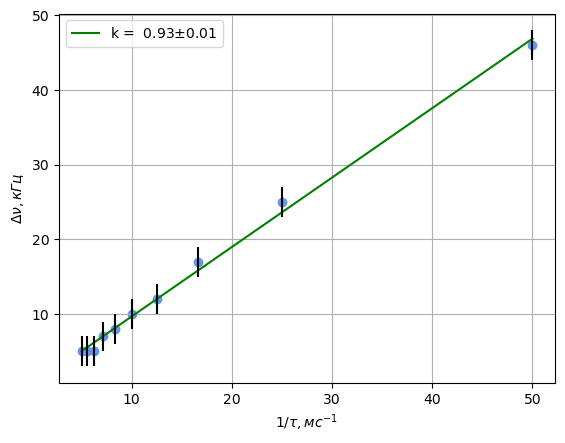
\includegraphics[width=8cm]{plot1.png}
        \caption{График зависимости $\Delta\nu(1 / \tau)$}
    \end{subfigure}
    \hfill
    \begin{subfigure}[b]{0.48\linewidth}
        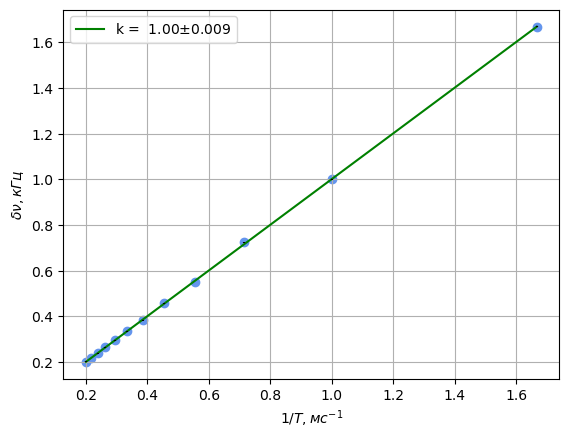
\includegraphics[width=8cm]{plot2.png}
        \caption{График зависимости $\delta\nu(1 /T)$}
    \end{subfigure}
\end{figure}


\begin{figure}[h!]
    \centering
    \begin{subfigure}[b]{0.48\linewidth}
        \centering
        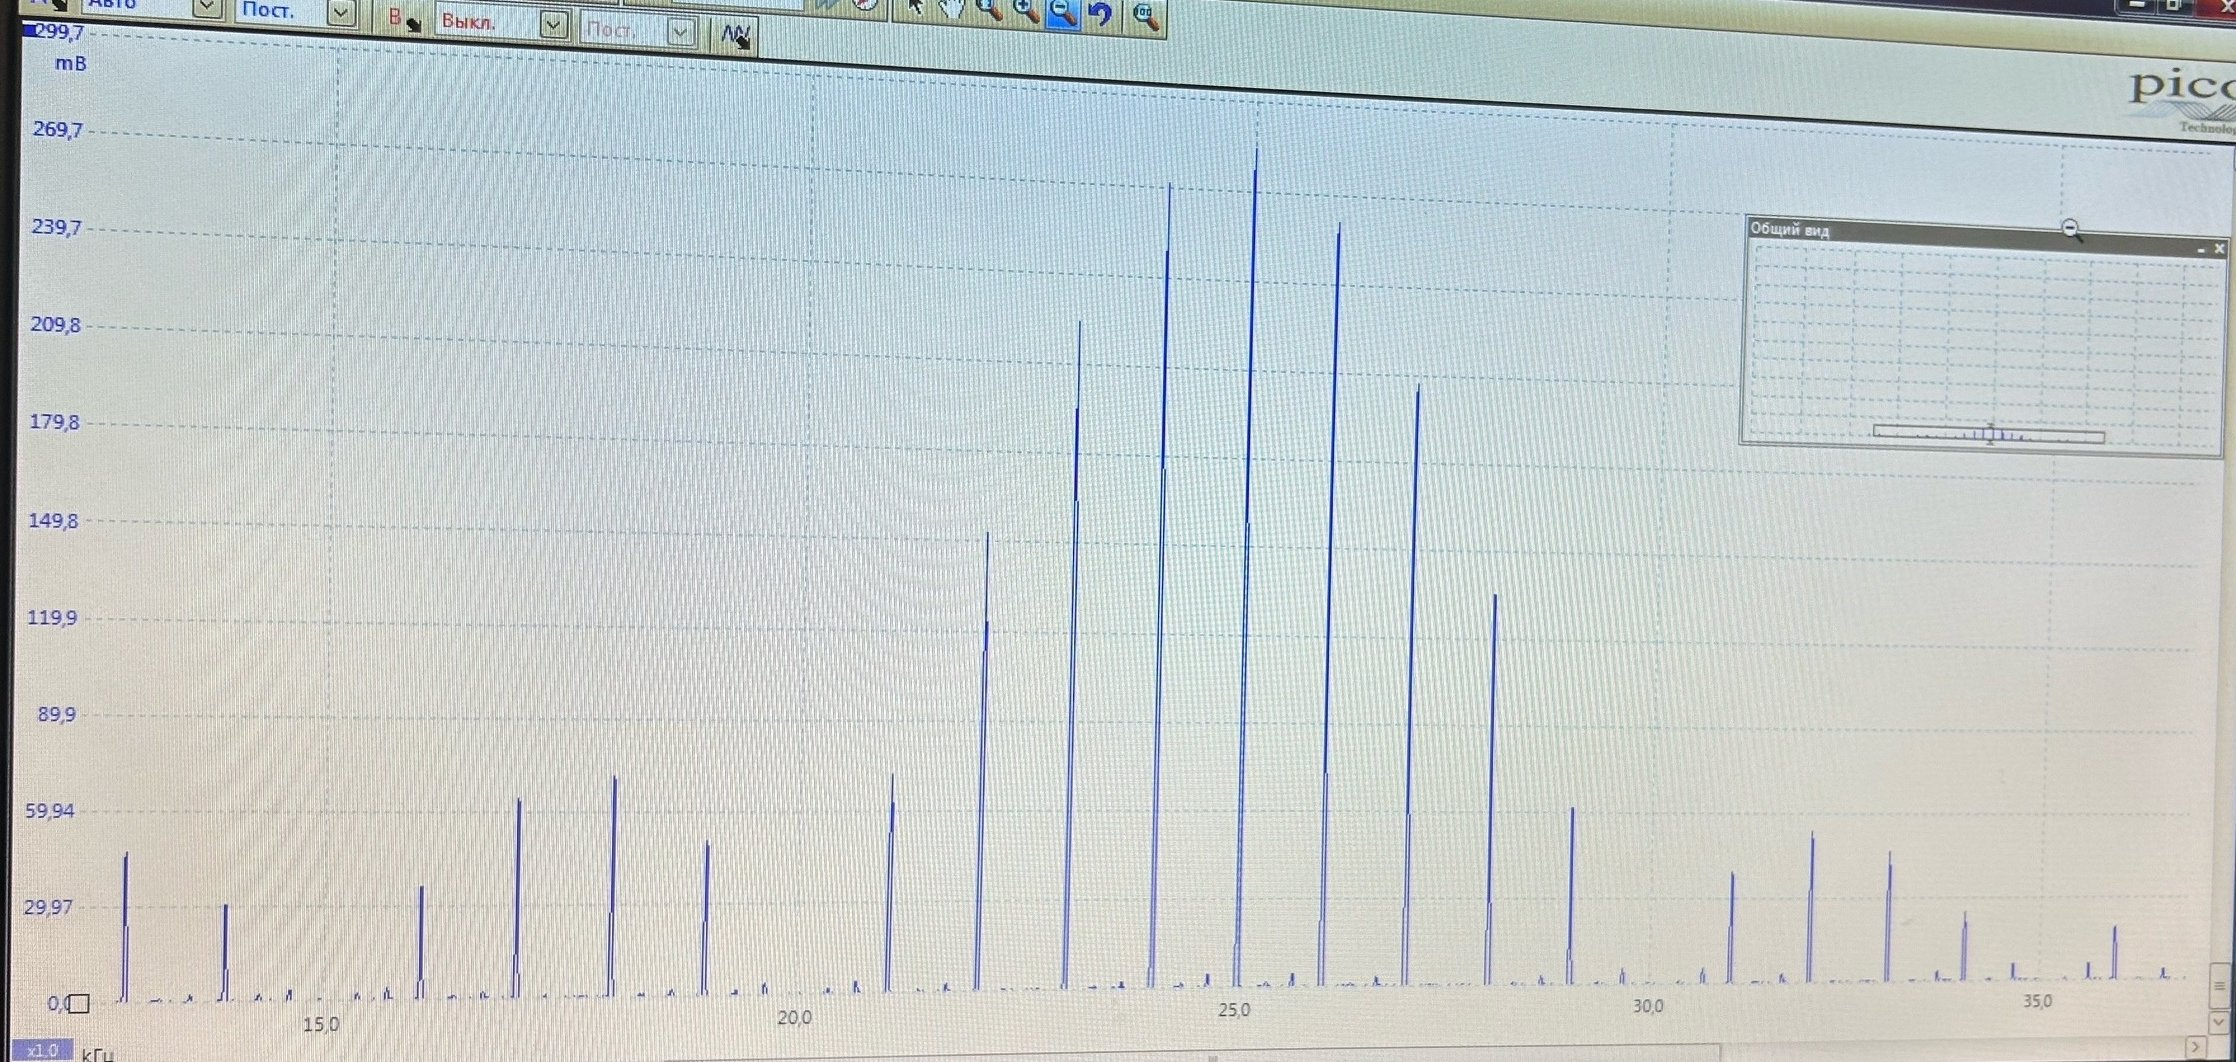
\includegraphics[width=8cm]{./images/tusgi/1_25_4_1.jpg}
        \caption{$\nu_0 = 25$кГц; $\Delta\nu = 9$ кГц; $\delta\nu = 1$ кГц}
    \end{subfigure}
    \hfill
    \begin{subfigure}[b]{0.48\linewidth}
        \centering
        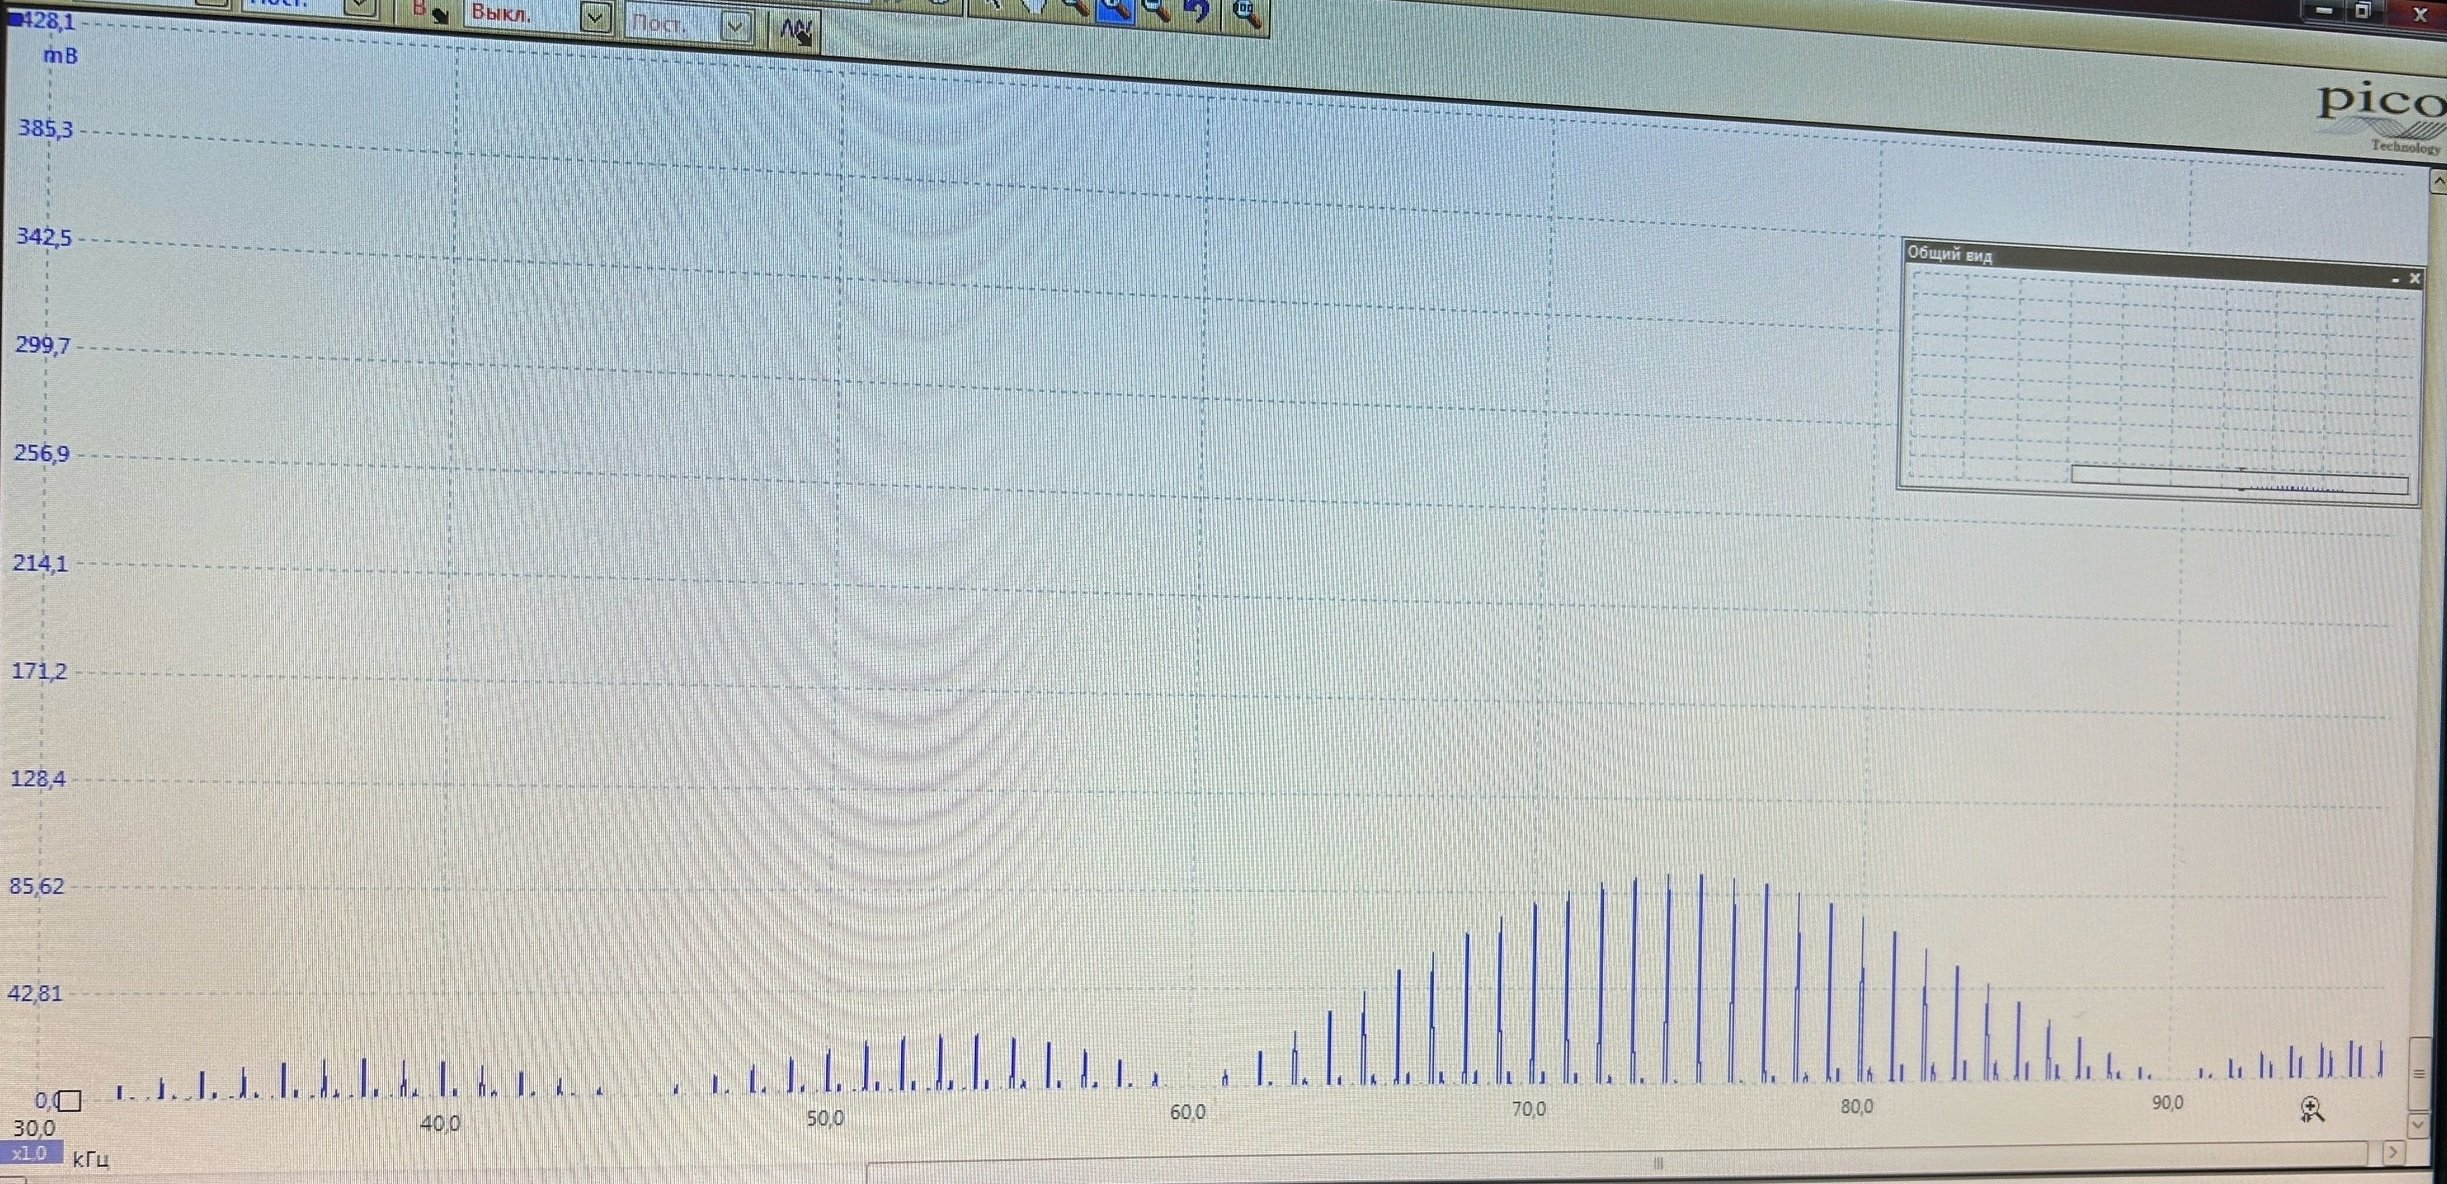
\includegraphics[width=8cm]{./images/tusgi/1_75_14_1.jpg}
        \caption{$\nu_0 = 75$кГц; $\Delta\nu = 5$ кГц; $\delta\nu = 1$ кГц}
    \end{subfigure}
    \vfill
    \begin{subfigure}{0.48\linewidth}
        \centering
        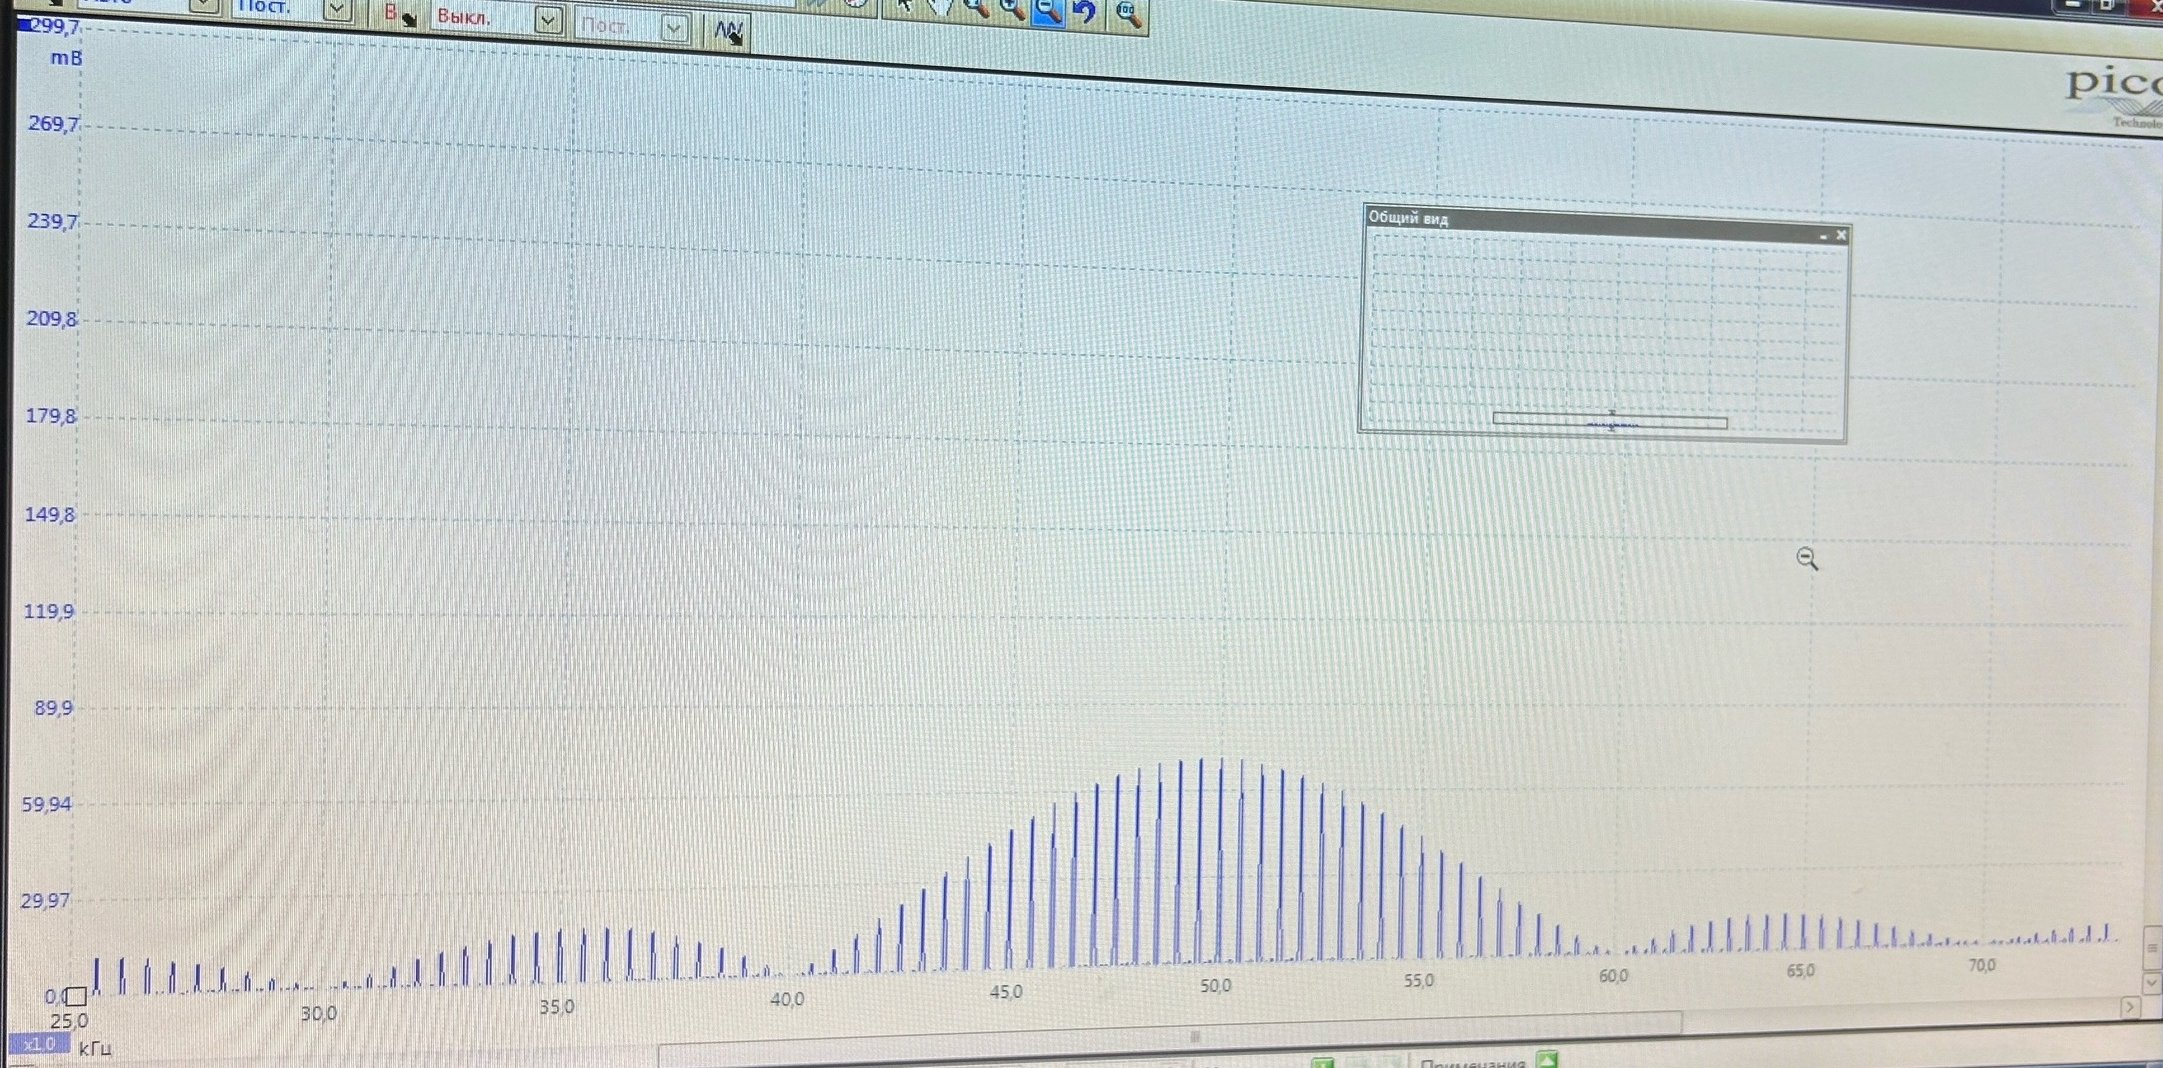
\includegraphics[width=8cm]{./images/tusgi/2_2_10_0-5.jpg}
        \caption{$T = 2$ мс; $\Delta\nu = 10$ кГц; $\delta\nu = 0.5$ кГц}
    \end{subfigure}
    \hfill
    \begin{subfigure}{0.48\linewidth}
        \centering
        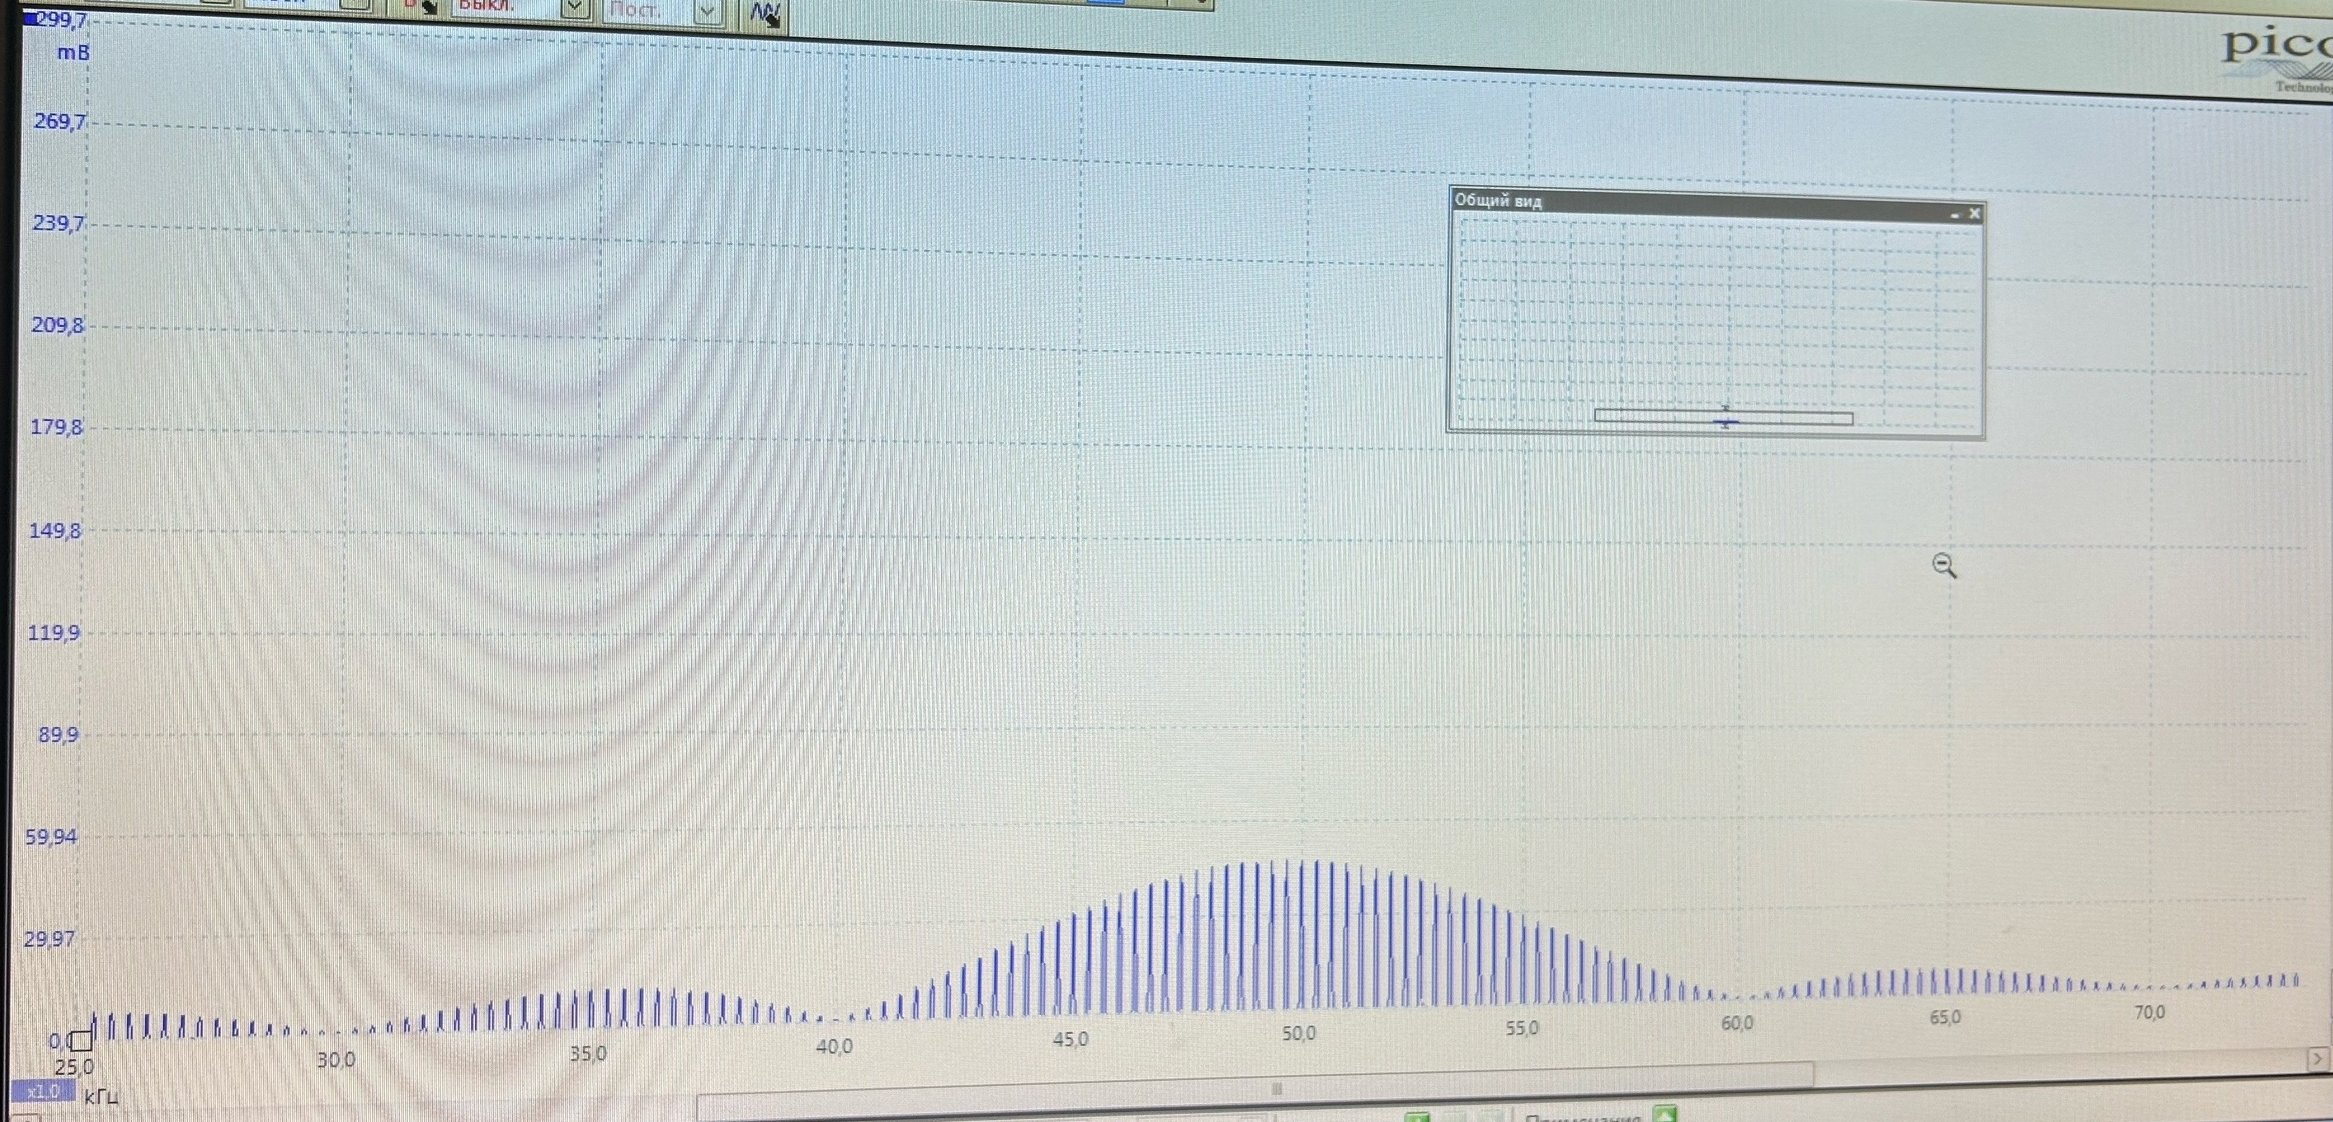
\includegraphics[width=8cm]{./images/tusgi/2_3_10_0-33.jpg}
        \caption{$T = 3$ мс; $\Delta\nu = 10$ кГц; $\delta\nu = 0.33$ кГц}
    \end{subfigure}
    \vfill
    \begin{subfigure}{0.48\linewidth}
        \centering
        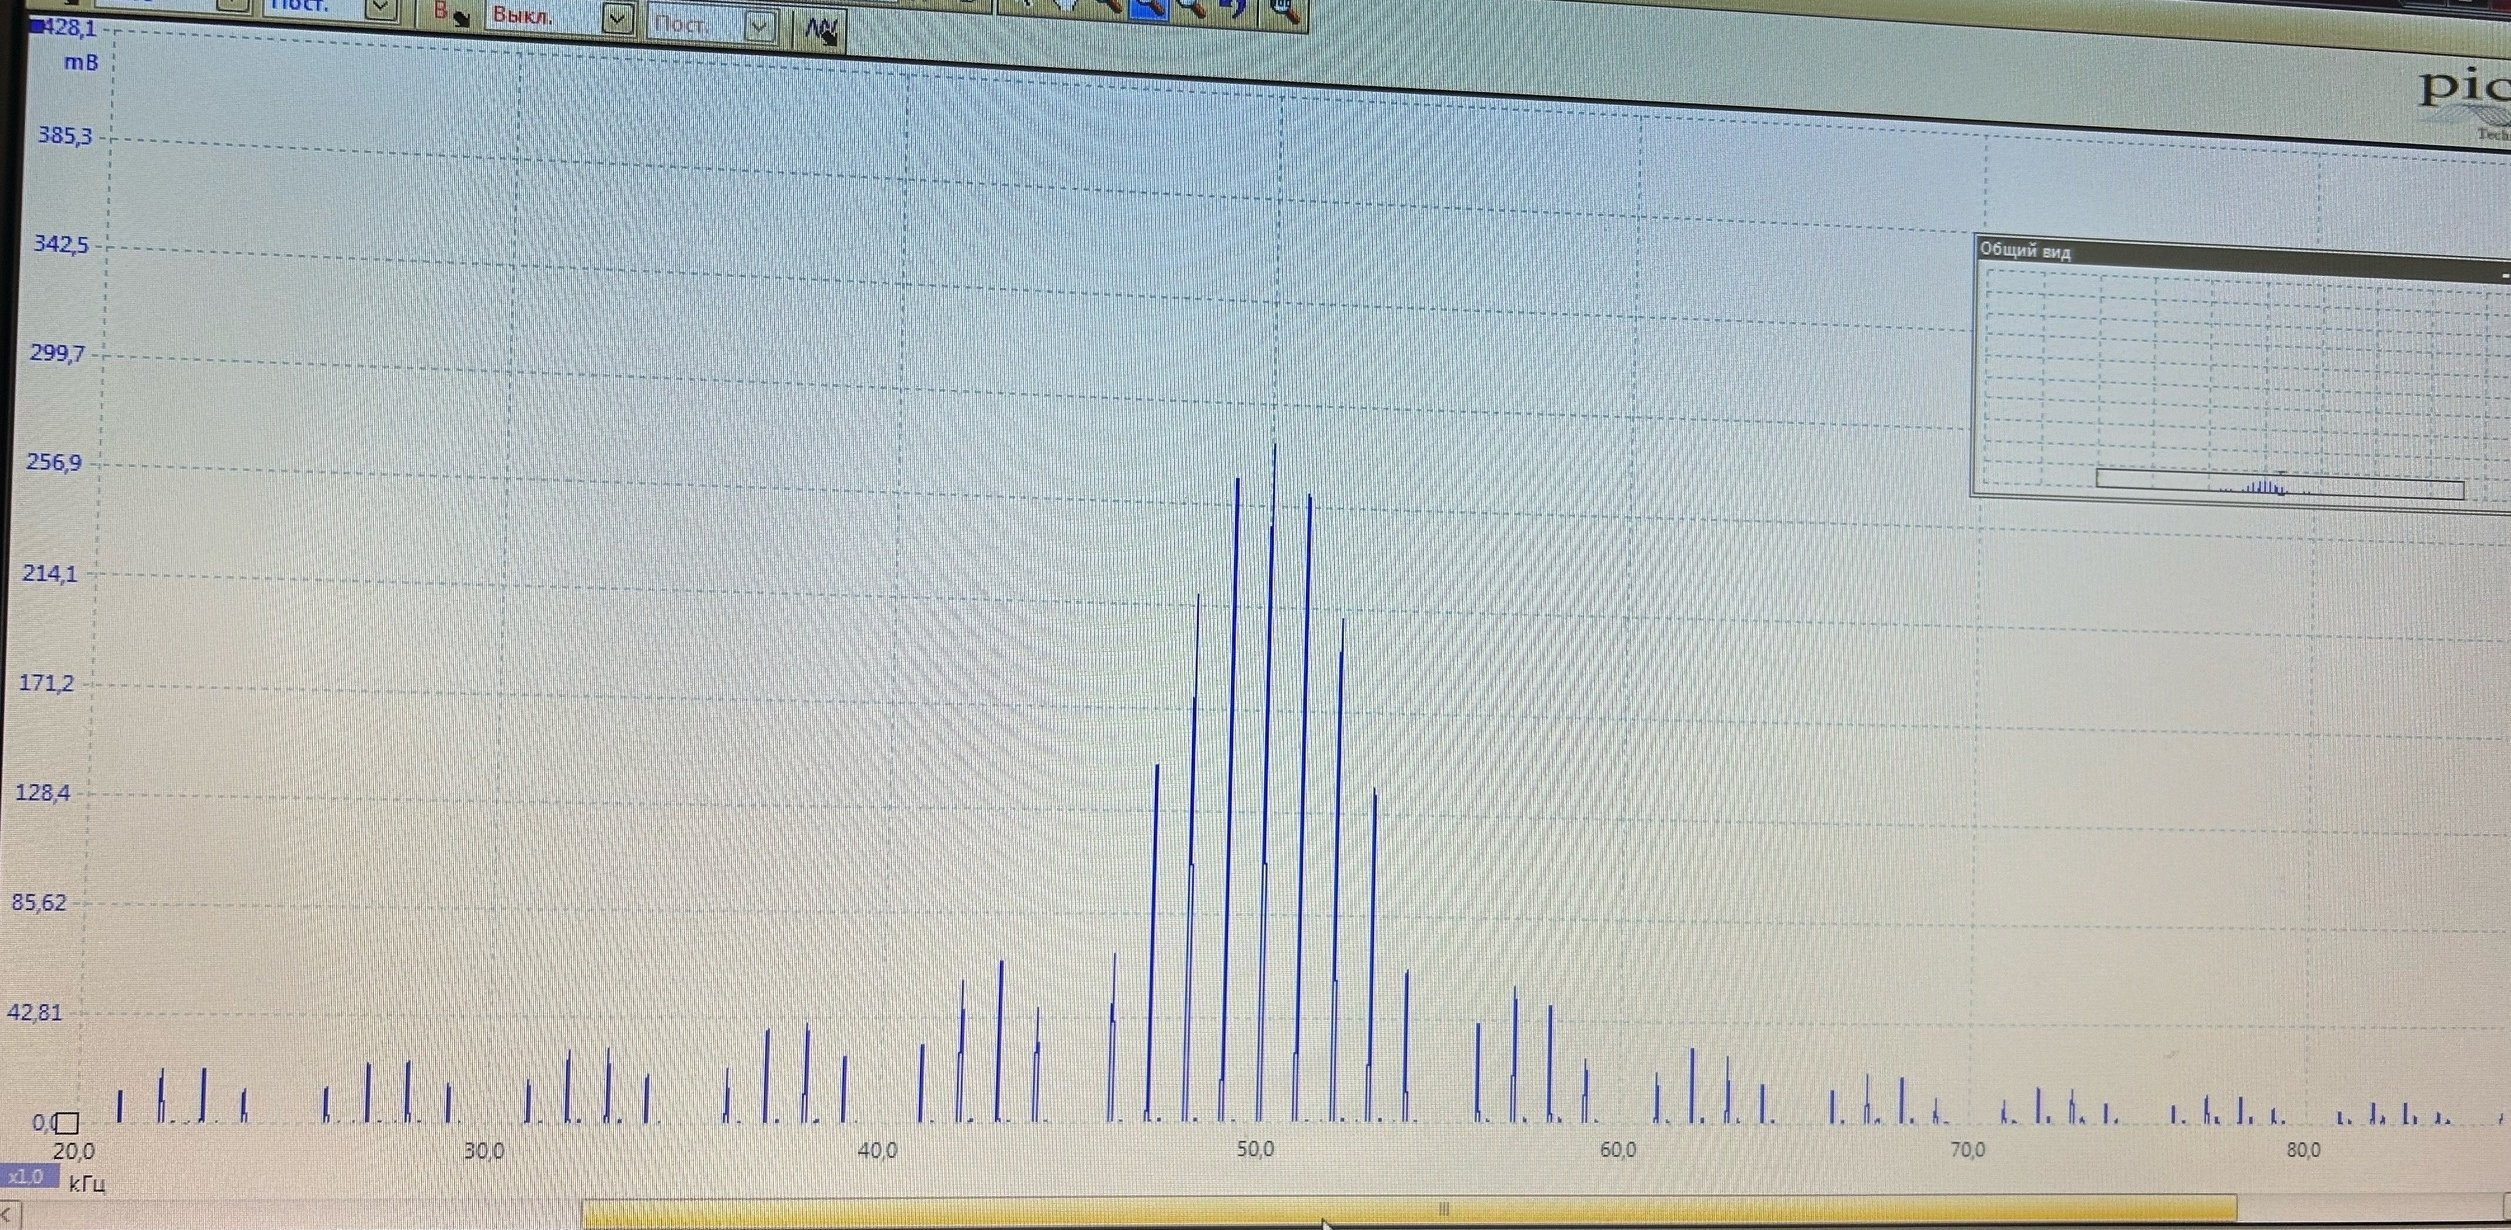
\includegraphics[width=8cm]{./images/tusgi/3_10_4_1.jpg}
        \caption{$N = 10$ шт; $\Delta\nu = 4$ кГц; $\delta\nu = 1$ кГц}
    \end{subfigure}
    \hfill
    \begin{subfigure}{0.48\linewidth}
        \centering
        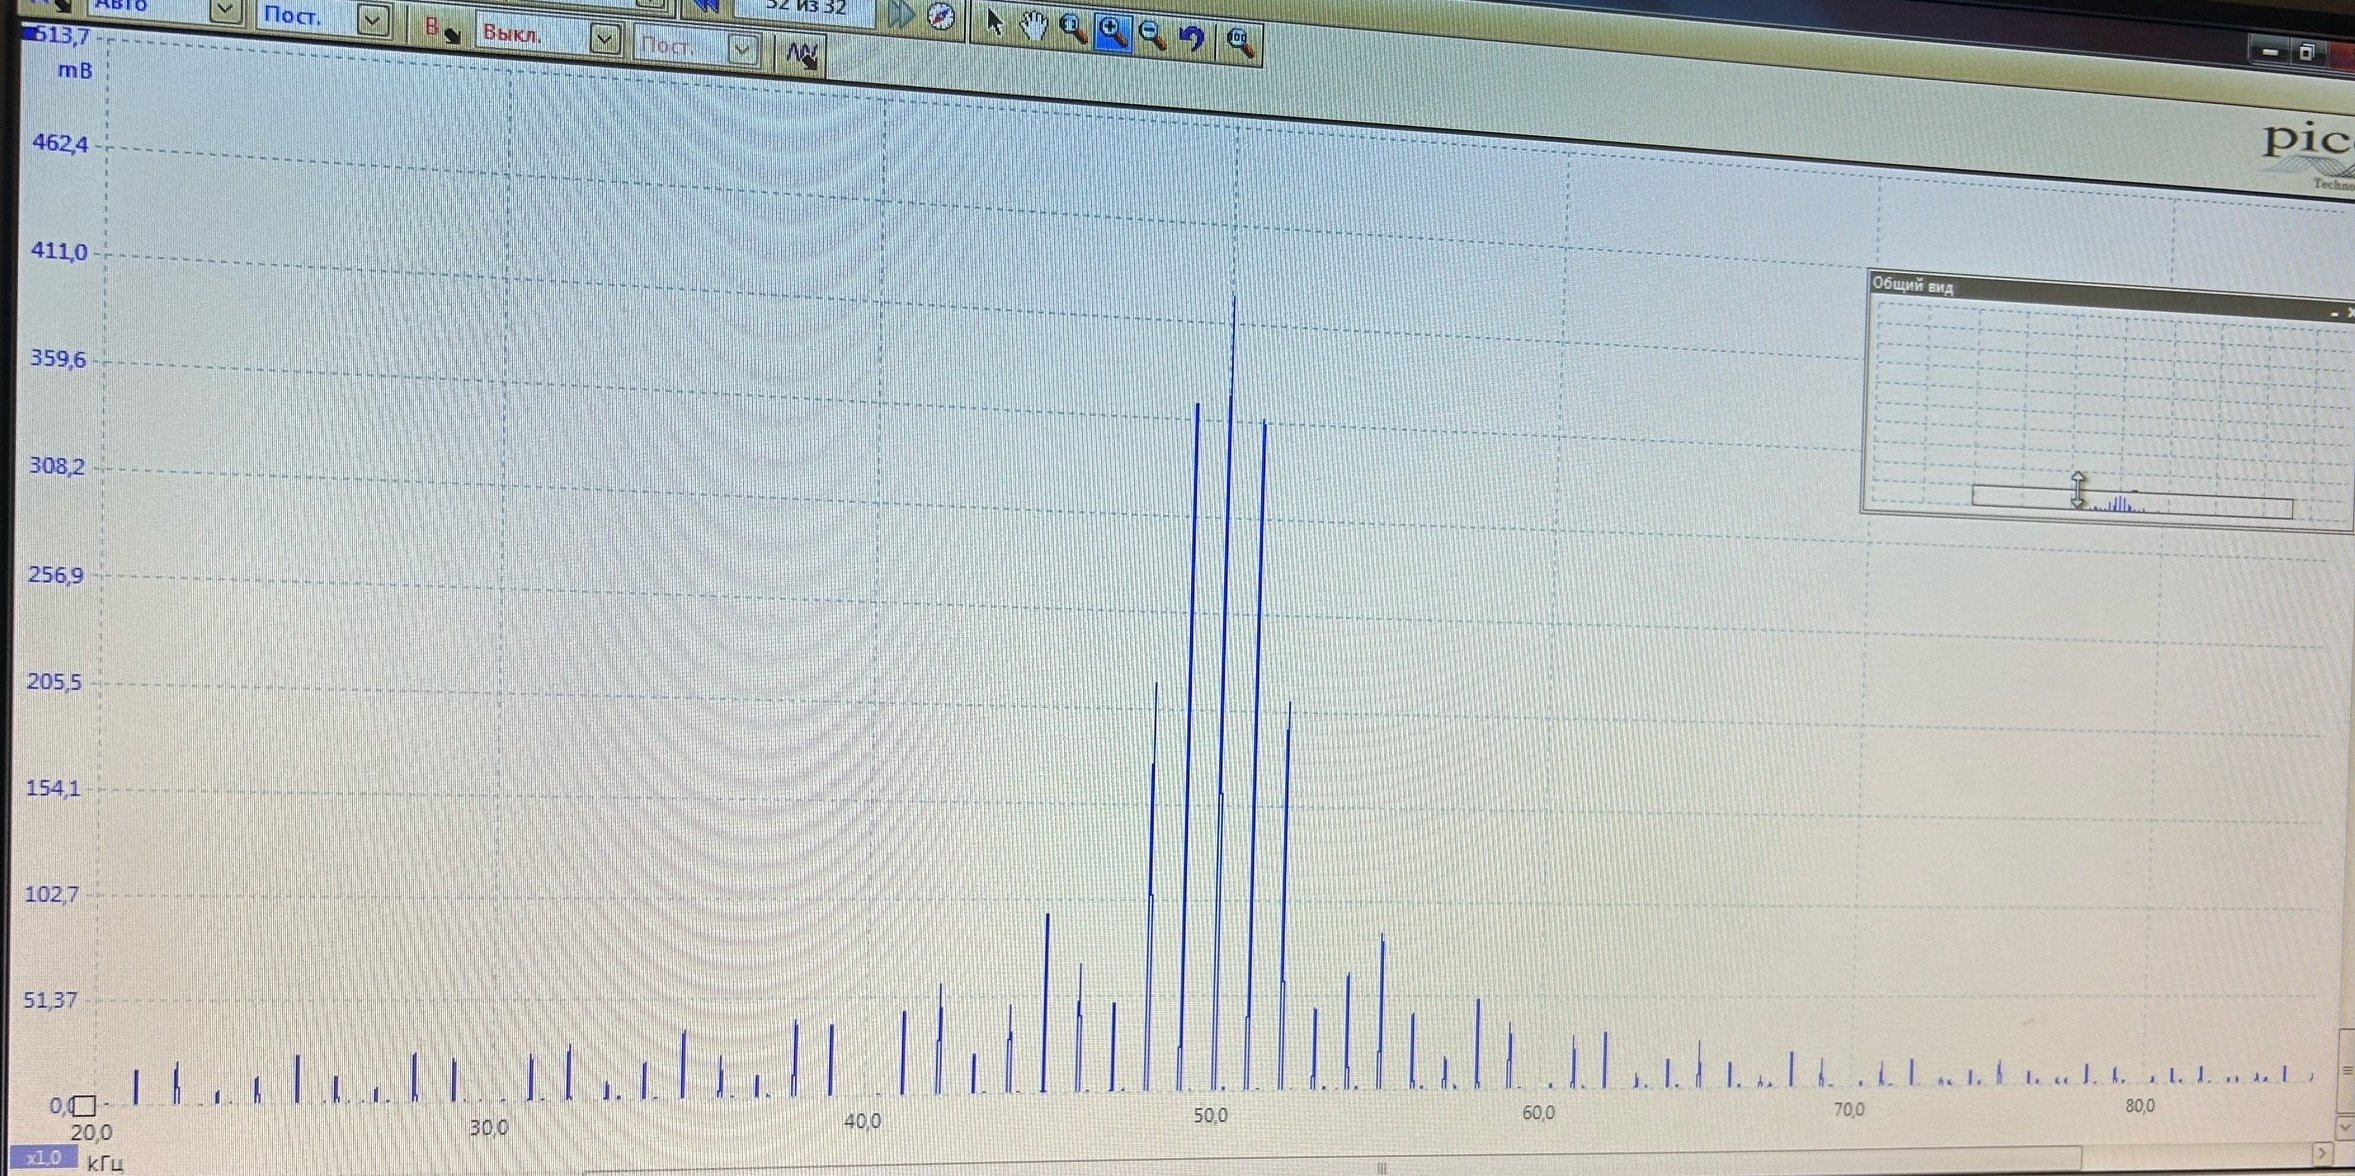
\includegraphics[width=8cm]{./images/tusgi/3_15_3_1.jpg}
        \caption{$N = 15$ шт; $\Delta\nu = 3$ кГц; $\delta\nu = 1$ кГц}
    \end{subfigure}
    \caption{Спектры синусоидального цуга при разных значениях параметров $\nu_0, N, T$\\Значения по умолчанию: $T$ = 1мс; $\nu_0$ = 50 кГц; $N$ = 5 шт}
\end{figure}

\newpage
\subsection*{Наблюдение спектра периодической последовательности цугов}
Обратное преобразование Фурье:
\begin{equation}
    f(t) = \frac{1}{2\pi}\int_{-\infty}^{\infty}F(\omega)e^{i\omega t}d\omega
\end{equation}

\noindent Прямое преобразование Фурье:
\begin{equation}
    F(t) = \int_{-\infty}^{\infty}f(t)e^{i\omega t}dt
\end{equation}
Теперь пусть $F_0(\omega)$ - спектр функции $f_0(t)$. Найдем спектр $F(\omega)$ функции $f(t) = f_0(t)\cos(\omega_0 t)$. $$f(t) = \frac{1}{2}f_0(t)e^{i\omega_0 t} + \frac{1}{2}f_0(t)e^{-i\omega_0 t}$$
Тогда из прямого преобразования Фурье:
$$\int_{-\infty}^{\infty}f_0(t)e^{-i(\omega - \omega_0)t}dt = F_0(\omega - \omega_0) \Rightarrow F(\omega) = \frac{1}{2}F_0(\omega - \omega_0) + \frac{1}{2}F_0(\omega + \omega_0)$$ 

Т.е исходный спектр сдвигается по оси частот на $\omega_0$ и домножается на 1/2.
\begin{figure}[h!]
    \centering
    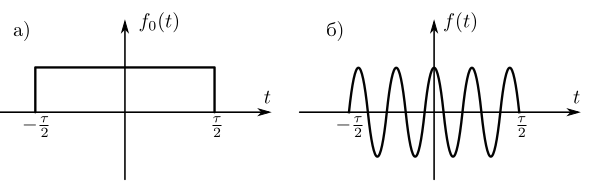
\includegraphics[width=12cm]{./images/прямоуг_син_сигнал.png}
    \caption{Прямоугольный и синусоидальный импульсы}
\end{figure}
\indent Найдем спектр обрывка синусоиды с частотой $\omega_0$ и длительностью $\tau$. Цуг может быть представлен как:
\begin{equation}
    f(t) = f_0(t)\cos(\omega_0 t)
\end{equation}
Тогда с учетом предыдущих выкладок получаем:
\begin{equation}
    F(\omega) = \frac{\tau}{2}\left [ \frac{\sin(\omega - \omega_0)\tau / 2}{(\omega - \omega_0)\tau/2} + \frac{\sin(\omega + \omega_0)\tau / 2}{(\omega + \omega_0)\tau/2}\right ]
\end{equation}

% \noindent\textbf{Теoрема смещения.} Найдем спектр $F(\omega)$ сигнала, смещенного по времени $f(t) = f_0(t - \tau)$, $f_0(t)$ - функция со спектром $F_0(\omega) = \hat{\mathcal{F}}[f_0]$. Преобразование Фурье:
% \begin{align}
%     F(\omega) = \hat{\mathcal{F}}[f(t)] = \int_{-\infty}^{\infty}f_0(t - \tau)e^{-i\omega t}dt \hspace{1cm}
%     t' = t - \tau\\ 
%     F(\omega) = \int_{-\infty}^{\infty}f_0(t')e^{-i\omega (t + \tau)}dt' = e^{-i\omega\tau}\cdot F_0(\omega)
% \end{align}
% Т.е смещение сигнала на $\tau$ приводит к умножению его спектра на $e^{-i\omega\tau}$.
Убедимся в справедливости соотношени неопределенности и теоремы смещения.
\begin{table}[!h]
    \centering
    \begin{tabular}{|c|c|c|c|c|c|}
        \hline
        $\Delta\nu$, кГц & 9 & 5 & 14 & 4 & 3 \\\hline
        $\tau = N / \nu_0$, мкс & 100 &200 & 66 & 200 & 300 \\\hline
        $\Delta\nu\cdot\tau$ & 0.9 & 1 & 0.924 & 0.8 & 0.9\\\hline
    \end{tabular}
    \caption{Проверка соотношения неопределенности}
\end{table}

\newpage
\subsection*{Исследование спектра амплитудно-модулированного сигнала}
Рассмотрим просейшее амплитудно-модулированное колебание:
\begin{align}
    f(t) = a(t)\cos(\omega_o t); \hspace{1cm} a(t) = a_0(1 + m\cos(\Omega t))
\end{align}
$m$ - клубина модуляции, связанная с максимальной и минимальной амплитудой:
\begin{align}
    m = \frac{a_{\text{max}} - a_{\text{min}}}{a_{\text{max}} + a_{\text{min}}}
\end{align}
$$ 
f(t) = a_0\cos\omega_0 t + \frac{ma_0}{2}\cos(\omega_0 + \Omega)t + \frac{ma_0}{2}\cos(\omega_0 - \Omega)t
$$
\begin{wrapfigure}{r}{0.6\linewidth}
    \centering
    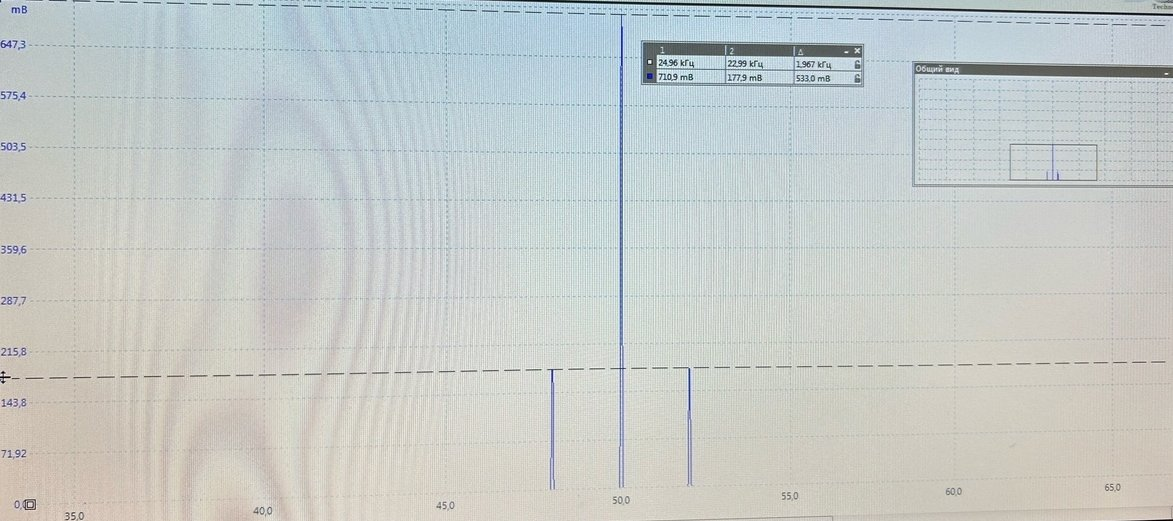
\includegraphics[width=8cm]{./images/m_50_nu_50.jpg}
    \caption{Амплитудная модуляция\\$\nu_0 = 50$ кГц; $\nu_{\text{мод}} = 2$ кГц; $m = 0.5$; $m_{\text{форм}}$ = 0.51 }
\end{wrapfigure}

Как видим, посчитанное значение глубины модуляции почти совпадает с заданным занчением в $50\%$.
\\\indent Теперь меняя на генераторе глубину модуляции, мы будем измерять отношение амплитуд боковой и основной спектральных линий.\\\\\\

Видим, что коэффициент прямой 1/2, что совпадает с теорией:
$a_{\text{бок}} / a_{\text{осн}} = \frac{ma_0 / 2}{a_0} = \frac{1}{2}m$
\begin{wrapfigure}[1]{l}{0.46\linewidth}
        \centering
        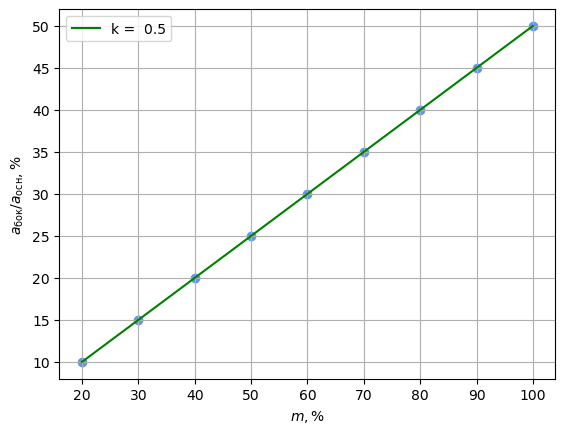
\includegraphics[width=8cm]{plot3.png}
        \caption{График зависимости $a_{\text{бок}} / a_{\text{осн}}$ от $m$}
\end{wrapfigure}
\newpage
\subsection*{Изучение фильтрации сигналов}
\textbf{Параметры RC-цепочки:} $R = 3$ кОм; $C = 1000$ пФ $\Rightarrow$ $\tau_{\text{RC}} = RC = 3$ мкс.

\begin{figure}[h!]
    \centering
    \begin{subfigure}[b]{0.48\linewidth}
        \centering
        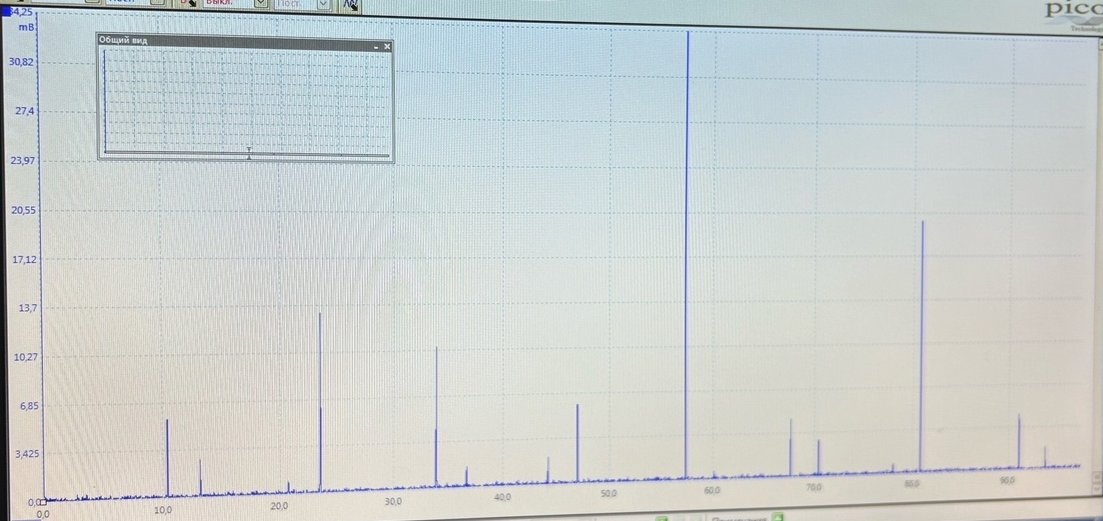
\includegraphics[width=8cm]{./images/T_x.jpg}
        \caption{$T = 3$ мкс}
    \end{subfigure}
    \hfill
    \begin{subfigure}[b]{0.48\linewidth}
        \centering
        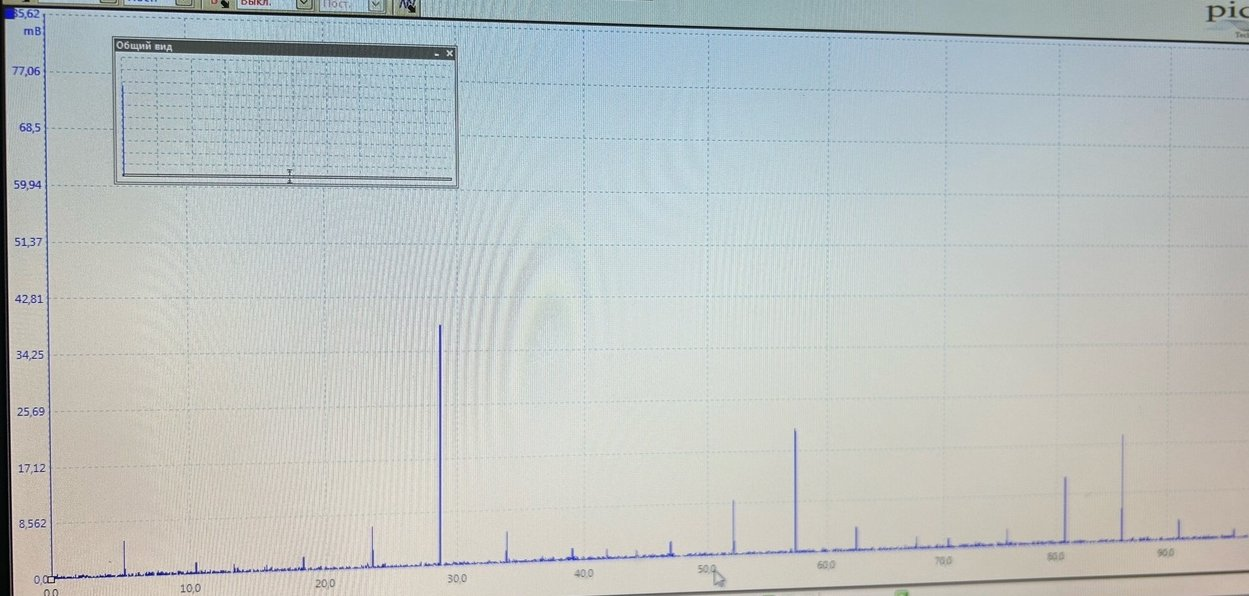
\includegraphics[width=8cm]{./images/T_6.jpg}
        \caption{$T = 6$ мкс}
    \end{subfigure}
    \vfill
    \begin{subfigure}[b]{0.48\linewidth}
        \centering
        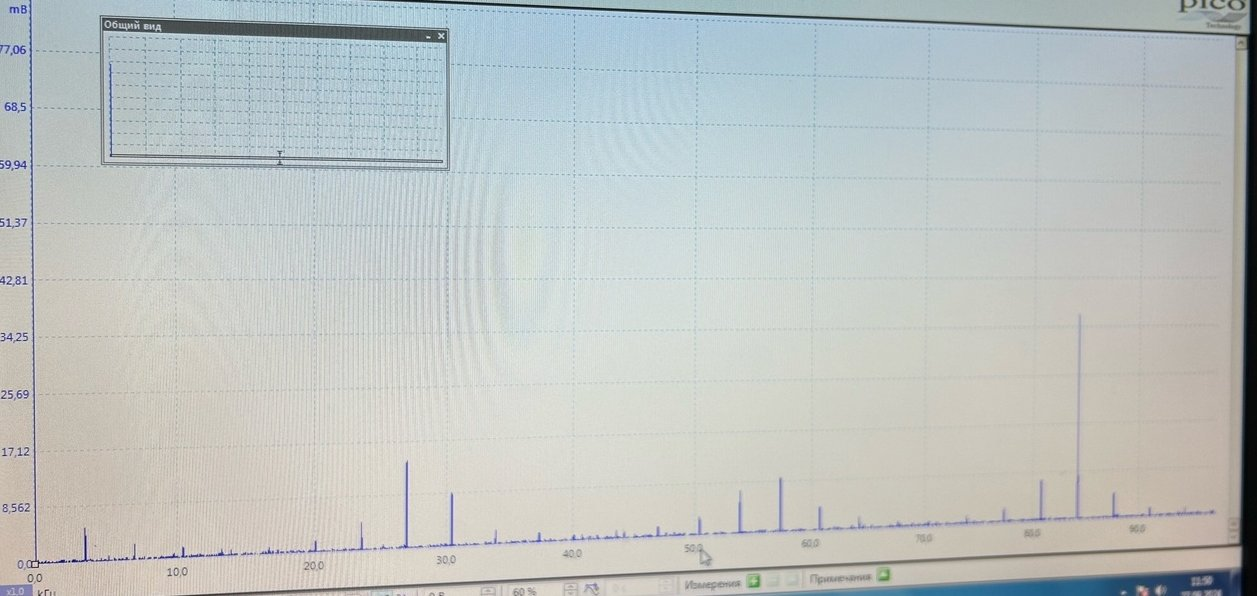
\includegraphics[width=8cm]{./images/T_9.jpg}
        \caption{$T = 9$ мкс}
    \end{subfigure}
    \hfill
    \begin{subfigure}[b]{0.48\linewidth}
        \centering
        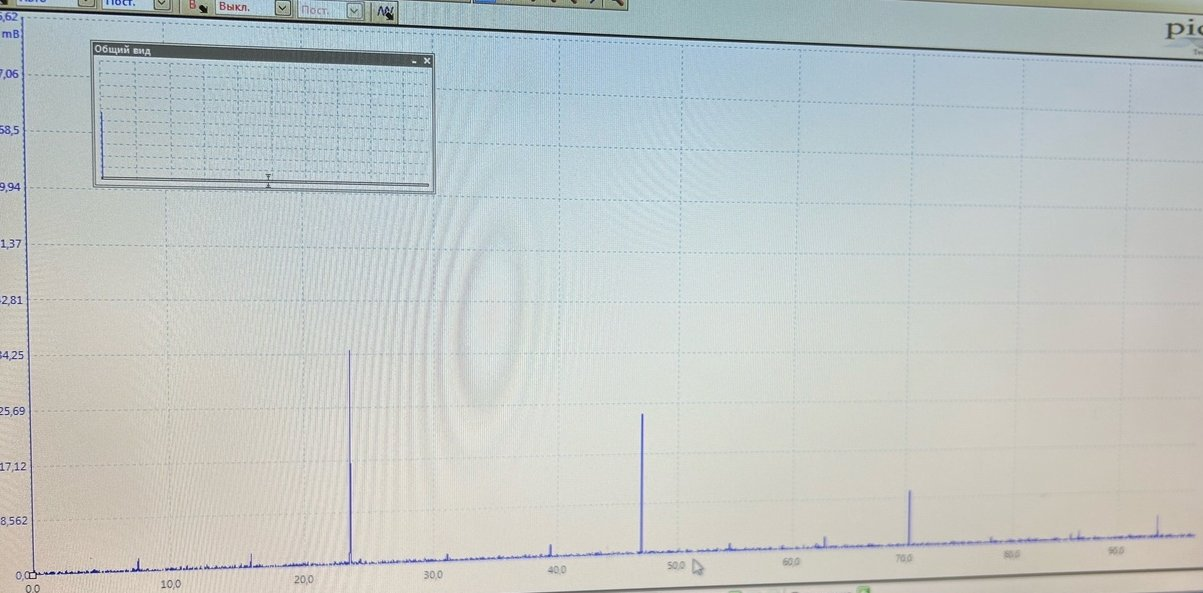
\includegraphics[width=8cm]{./images/T_1.jpg}
        \caption{$T = 1$ мкс}
    \end{subfigure}
    \caption{Спектры "фильтрованного" сигнала $RC-цепочки$ при различных значениях $T$}
\end{figure}

\begin{table}[h!]
    \centering
    \begin{tabular}{|c|c|c|c|c|c|c|c|}
        \hline
        $n$ & 1 & 2 & 3 & 4 & 5 & 6 & 7\\\hline
        $a_n^{\text{ф}}/a_n^{\text{исх}}$ & 0.0128& 0.0094& 0.006& 0.004& 0.0026& 0.0025& 0.0021\\\hline
    \end{tabular}
\end{table}

\begin{figure}[!h]
\begin{subfigure}[b]{0.48\linewidth}
    \centering
    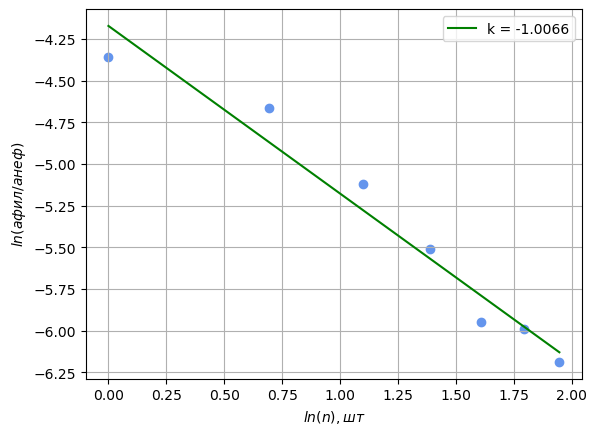
\includegraphics[width=8cm]{plot5.png}
    \caption{Зависимость $K(n)$ в логарифмических координатах}
\end{subfigure}
\hfill
\begin{subfigure}[b]{0.48\linewidth}
    \centering
    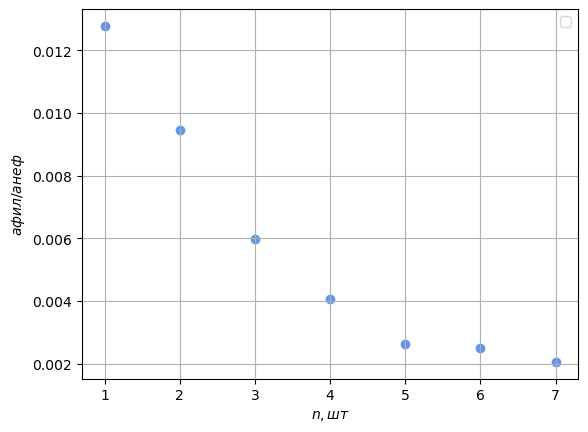
\includegraphics[width=8cm]{plot4.png}
    \caption{Cхема фильтрации сигналов}
\end{subfigure}
\end{figure}
Из логарифмического графика видим, что $K$ обратно пропорционален $n$. Действительно $K = \frac{1}{\tau_{\text{RC}}}\int_{0}^{t} f(t)dt = \frac{t}{\tau_{\text{RC}}}$ т.е обртно пропорционально частоте $\nu = n\nu_0$.
\newpage
\begin{figure}[!h]
\begin{subfigure}[b]{0.48\linewidth}
    \centering
    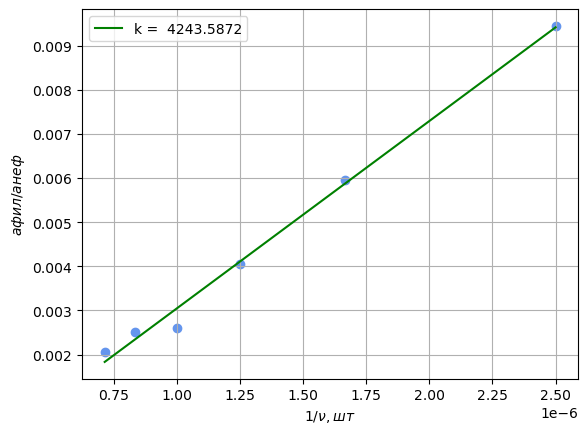
\includegraphics[width=8cm]{plot6.png}
    \caption{Зависимость $K(1/n)$}
\end{subfigure}
\hfill
\begin{subfigure}[b]{0.48\linewidth}
    \centering
    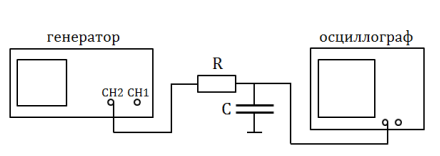
\includegraphics[width=8cm]{./images/setup.png}
    \caption{Cхема фильтрации сигналов}
\end{subfigure}
\end{figure}
По графику найдем экспериментально $\tau_{\text{RC}} = \frac{1}{2\pi\nu_0 k} \approx 37\pm26$ мкс, что почти в 10 раз больше теоретического значения в 3мкс. 

\subsection*{Результаты и выводы}
1)Исследуя спектр прямоугольных импульсов, сравнили теоретическое и экспериментальные значения соотношения амплитуд и проверили формулу неопределенности. Результаты хорошо совпали с теорией.\\ 
2)Наблюдали спектр периодической последовательности цугов и убедились в теореме смещения. Центр спектра смещался на $\nu_0$.\\ 
3)Исследyя спектр амплитудно-модулированного сигнала, убедились в справедливости изложенной теории (отношение боковой и основной гармоники равно половине глубины модуляции)\\
4)Изучали фильтрацию сигналов на $RC$-цепочке. Проверили экспериментально, что коэффициент фильтрации $K$ обратно пропорционален номеру гармоники. Однако экспериментально полученное из графиков значение $\tau_{\text{RC}}$ значительно отличается от теор.значения. Даже с учетом погрешности в 70\%.


